\chapter{引导与可控生成}\label{ch:guidance}
扩散模型是强大的生成式框架。在无条件设定下，目标是学习 $p_{\text{data}}(\rvx)$ 并在没有外部输入的情况下生成样本。

然而，许多应用需要\emph{条件生成}，即输出须满足用户指定的标准。这可以通过对无条件模型进行引导，或者直接学习条件分布 $p_0(\rvx | \rvc)$ 来实现，其中条件 $\rvc$（例如标签、文本描述或草图）引导整个过程。

本章基于条件分数的一个原则性视角，该视角将条件分数分解为一个\emph{无条件方向}和一个\emph{引导方向}：前者在保持真实性的同时将样本推向所给条件。我们将解释为何引导是必不可少的，说明条件分数如何作为统一的控制接口，并综述近似引导项的多种方法。随后，我们将区分\emph{控制}（满足条件）与\emph{对齐}（在给定条件下满足人类偏好），并阐述如何将偏好纳入同一框架。最后，我们讨论在无需额外奖励模型（即一个学习得到的评分器，它对与人类偏好更一致的输出赋予更高的值）的情况下直接优化偏好。




\clearpage
\newpage

\section{引言}\label{sec:prologue-guidance}


\begin{figure}[th!]
    \centering
    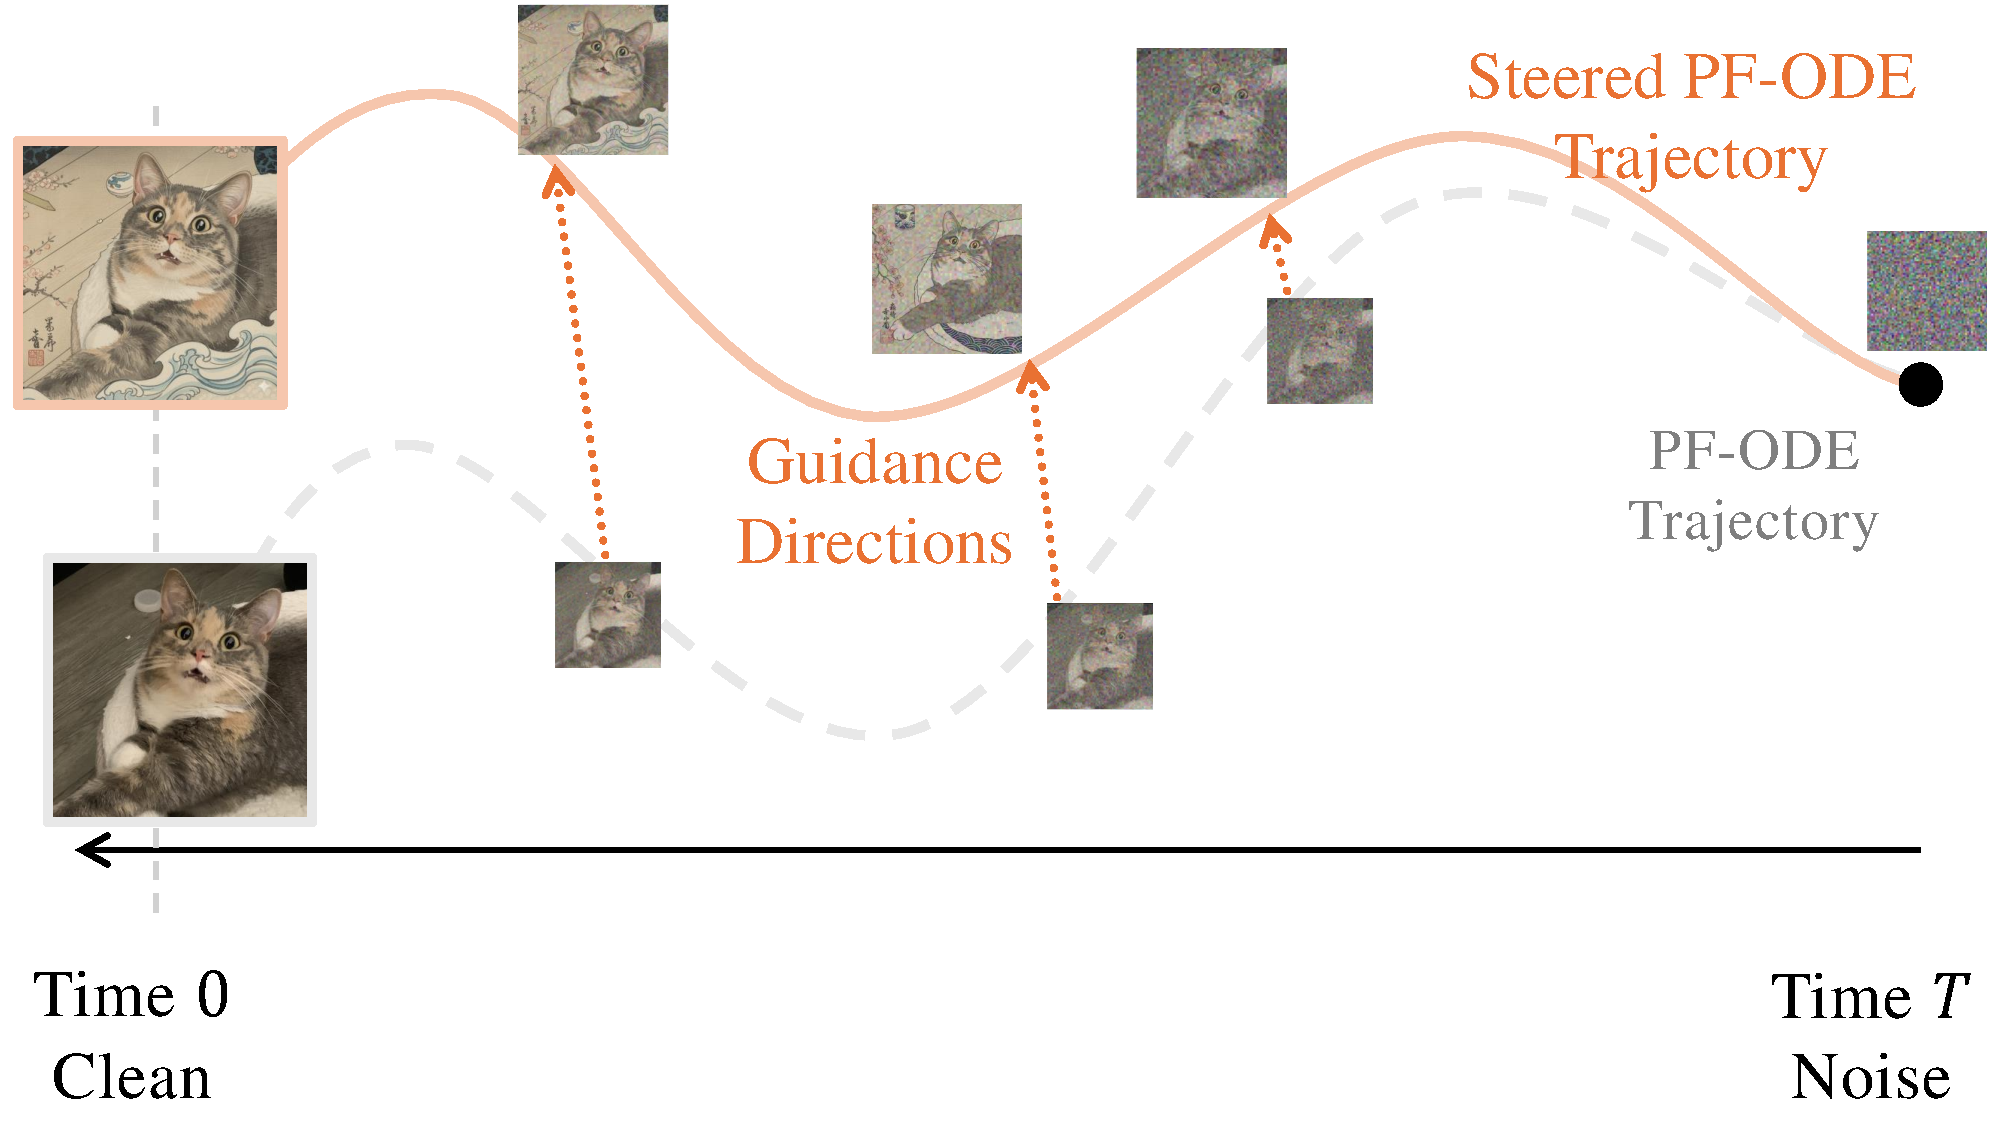
\includegraphics[width=\linewidth]{Images/PartC/guidance.pdf}
\caption{\textbfs{引导扩散采样的示意图。}
逆向时间 PF-ODE 采样从右侧的纯噪声（$t = T$）开始，逐步演化为左侧（$t = 0$）的清晰样本。
在此过程中，由 $w_t$ 加权的引导方向 $\nabla_{\rvx_t}\log \tilde{p}_t(\rvc |\rvx_t)$ 按照下式修改速度场：
$\nabla_{\rvx_t}\log p_t(\rvx_t) + w_t\,\nabla_{\rvx_t}\log \tilde{p}_t(\rvc |\rvx_t)$。
这些额外的方向在样本由粗到细逐步精化的同时，将轨迹引向目标属性（日本绘画风格）。
\figcredit{由作者绘制。}}
    \label{fig:guidance}
\end{figure}


扩散模型的生成过程以由粗到细的方式进行，为可控生成提供了灵活的框架。在每一步中，少量噪声被移除，样本变得更加清晰，逐渐显现出更多的结构和细节。这一特性使我们可以对生成过程进行控制：通过在所学到的、随时间变化的速度场上添加一个引导项，我们可以引导生成轨迹反映用户的意图。

扩散模型中基于引导的采样的一个原则性基础是条件分数的贝叶斯分解。对于每个噪声水平 $t$，
\begin{mdframed}
\begin{align}
\nabla_{\rvx_t}\log p_t(\rvx_t |\rvc)
=
\underbrace{\nabla_{\rvx_t}\log p_t(\rvx_t)}_{\text{无条件方向}}
+
\underbrace{\nabla_{\rvx_t}\log p_t(\rvc |\rvx_t)}_{\text{引导方向}}.
\label{eq:guidance_bayes}
\end{align}
\end{mdframed}
这一恒等式表明，条件采样可以通过在无条件分数之上添加一个引导项 $\nabla_{\rvx_t}\log p_t(\rvc |\rvx_t)$ 来实现。由于 $p_t(\rvc |\rvx_t)$ 通常因为要对 $\rvx_0$ 进行边缘化而难以处理，各种可控生成方法（例如分类器引导~\citep{dhariwal2021diffusion}、通用的免训练引导~\citep{ye2024tfg}）都可以解释为对该引导项的不同近似。

一旦获得了这样的近似，采样只需用条件分数替代无条件分数即可。利用 \Cref{eq:guidance_bayes}，PF-ODE 变为
\begin{align}\label{eq:condition_prob_ode}
\begin{aligned}
    \frac{\diff \mathbf{x}(t)}{\diff t} &= f(t)\mathbf{x}(t) - \frac{1}{2} g^2(t) \underbrace{\nabla_{\rvx_t} \log p_t(\rvx(t) |\rvc)}_{\text{条件分数}} \\
    &= f(t)\mathbf{x}(t) - \frac{1}{2} g^2(t) \Big[ \nabla_{\rvx_t} \log p_t(\rvx(t)) + \nabla_{\rvx_t} \log p_t(\rvc |\rvx(t)) \Big].
\end{aligned}
\end{align}
我们强调，引导这些随时间变化的向量场从根本上依赖于它们的线性性，因此下文以分数预测形式给出的讨论，可通过 \Cref{eq:predictions-equivalence} 中的线性关系自然地推广到 $\rvx$-、$\beps$- 和 $\rvv$-预测。

\paragraph{引导方向的具体形式。}
\begin{enumerate}[leftmargin=*]
\item \textbfs{分类器引导（CG）。} 在 \Cref{sec:cg} 中，分类器引导（CG）在加噪数据 $\rvx_t$（通过在水平 $t$ 上破坏带标签的干净样本得到）上训练一个时间条件分类器
$p_{\bpsi}(\rvc | \rvx_t, t)$。在采样时，其输入梯度提供引导项：
\[
\nabla_{\rvx_t}\log p_{\bpsi}(\rvc | \rvx_t, t)
 \approx  \nabla_{\rvx_t}\log p_t(\rvc | \rvx_t),
\]
随后将其加到无条件分数上~\citep{dhariwal2021diffusion}。
\item \textbfs{无分类器引导（CFG）。} 在 \Cref{sec:cfg} 中，CFG 直接训练单个条件模型
\[
\rvs_{\bphi}(\rvx_t,t,\rvc) \approx \nabla_{\rvx_t}\log p_t(\rvx_t|\rvc),
\]
其中无条件模型是通过在部分训练步骤中以一个特殊的空标记随机替换条件来联合学习的。
\item \textbfs{免训练（替代）引导。}  条件分布 $p_t(\rvc| \rvx_t)$ 通常难以处理，因为它需要对干净隐变量 $\rvx_0$ 进行边缘化：
\[
p_t(\rvc| \rvx_t)
= \int p(\rvc| \rvx_0)  p(\rvx_0| \rvx_t)  \mathrm d\rvx_0,
\]
而且在典型应用中，至少有一个因子是未知的，使得该积分难以计算。

在 \Cref{subsec:tfg} 中，免训练（基于损失的）引导避免直接评估条件似然 $p_t(\mathbf{c}| \mathbf{x}_t)$。
相反，它引入一个现成的损失 $\ell(\mathbf{x}_t,\mathbf{c};t)$
并将替代条件分布 $\widetilde p_t(\mathbf{c}|\mathbf{x}_t) $ 定义为
\[
\widetilde p_t(\mathbf{c}|\mathbf{x}_t) \propto \exp\!\big(-\tau\,\ell(\mathbf{x}_t,\mathbf{c};t)\big),
\quad \tau>0,
\]
它充当一个伪似然。
这一表述规避了计算真实条件似然的困难，同时仍然可以通过所选损失的梯度实现引导。其条件分数仅由带有 $\tau$ 的损失梯度计算：
\[
\nabla_{\rvx_t}\log \widetilde p_t(\rvc|\rvx_t)
= -\tau \nabla_{\rvx_t}\ell(\rvx_t,\rvc; t).
\]
这一项以引导权重 $w_t$ 加到无条件分数上：
\[
  \nabla_{\rvx_t}\log p_t(\rvx_t)
 + w_t \bigl[-\tau \nabla_{\rvx_t}\ell(\rvx_t,\rvc; t)\bigr].
\]
这恰好是 \emph{倾斜}密度 $\widetilde p_t^{\mathrm{tilt}}(\rvx_t| \rvc)$ 的分数，定义为：
\[
\widetilde p_t^{\mathrm{tilt}}(\rvx_t| \rvc) \propto  p_t(\rvx_t) \widetilde p_t(\rvc| \rvx_t)^{w_t}
 \propto  p_t(\rvx_t) \exp\!\big(-w_t\tau \ell(\rvx_t,\rvc; t)\big).
\]
在实践中，我们将 \Cref{eq:condition_prob_ode} 中采样的条件分数替换为该倾斜分数，并求解所得的 ODE 来抽取样本。

鉴于此，分类器引导只是用一个学习得到的分类器 $\widetilde p_t(\mathbf{c}|\mathbf{x}_t):=p_{\bpsi^\times}(\rvc| \rvx_t,t)$ 实现的替代引导，即：
\[
\ell(\rvx_t,\rvc; t) = -\log p_{\bpsi^\times}(\rvc| \rvx_t,t), \quad \tau=1.
\]

引导对采样轨迹的影响如 \Cref{fig:guidance} 所示。

所有这些技术同样可以叠加到条件模型之上，
从而允许在生成过程中注入额外的控制信号。

\end{enumerate}
\rmkb{引导 PF-ODE（一般而言）\emph{并不}从倾斜分布族中采样。
即便分数完全精确、ODE 积分也完全精确，将分数替换为\emph{倾斜}分数并不能使时间 $t$ 的边缘分布等于
$\{\widetilde p_t^{\mathrm{tilt}}(\cdot|\rvc)\}_{t\in[0,1]}$，也不能使终止分布等于
$\widetilde p_0^{\mathrm{tilt}}(\cdot|\rvc)$。

定义
\[
\rvv_t^{\mathrm{orig}} = \rvf - \tfrac12 g^2(t) \nabla \log p_t, \quad
\rvh_t(\rvx)=e^{-w_t\tau \ell(\rvx,\rvc;t)}, \quad
\widetilde p_t^{\mathrm{tilt}}=\tfrac{p_t \rvh_t}{Z_t}.
\]
引导后的 PF-ODE 使用
\[
\rvv_t^{\mathrm{tilt}} = \rvf - \tfrac12 g^2(t) \nabla \log \widetilde p_t^{\mathrm{tilt}}
= \rvv_t^{\mathrm{orig}} - \tfrac12 g^2(t) \nabla \log \rvh_t.
\]

如果 $\widetilde p_t^{\mathrm{tilt}}$ 是真实的边缘分布，它们应满足
\[
\partial_t \widetilde p_t^{\mathrm{tilt}} + \nabla\!\cdot(\widetilde p_t^{\mathrm{tilt}} \rvv_t^{\mathrm{tilt}})=0.
\]
但直接计算得到残差
\begin{align*}
    &\partial_t \widetilde p_t^{\mathrm{tilt}} + \nabla \cdot(\widetilde p_t^{\mathrm{tilt}}  \rvv_t^{\mathrm{tilt}})
\\= &\widetilde p_t^{\mathrm{tilt}} \Big[ \partial_t \log \rvh_t
+ \rvv_t^{\mathrm{orig}} \cdot\nabla \log \rvh_t
- \tfrac12 g^2(t) \big(\Delta \log \rvh_t + \|\nabla \log \rvh_t\|^2 \big)
- \tfrac{Z_t'}{Z_t} \Big].
\end{align*}

因此，$\widetilde p_t^{\mathrm{tilt}}$ 与 PF-ODE 的边缘分布相吻合，当且仅当对所有 $\rvx$ 括号中的项为零，即
\[
\partial_t \log \rvh_t + \rvv_t^{\mathrm{orig}} \cdot\nabla \log \rvh_t
= \tfrac12 g^2(t)\big(\Delta \log \rvh_t + \|\nabla \log \rvh_t\|^2\big) + \tfrac{Z_t'}{Z_t}.
\]
这一条件在 $w_t\equiv 0$（无条件生成）时平凡地成立，但对
$\rvh_t(\rvx)=e^{-w_t\tau\ell(\rvx,\rvc;t)}$ 几乎从不成立，除非 $w_t$ 或 $\ell$ 处于非常特殊的情况。因此，一般而言
$\{\widetilde p_t^{\mathrm{tilt}}\}$ \emph{并非} PF-ODE 的边缘分布，终止样本\emph{并不}服从 $\widetilde p_0^{\mathrm{tilt}}(\rvx_0|\rvc)$ 分布。这一视角在精神上也与 \citep{lai2023fp} 相关。


对于希望超越这种启发式引导的读者，基于校正的方法~\citep{skreta2025feynman}，例如 Feynman--Kac 校正子，旨在显式地补偿引导后的动力学与所期望的倾斜分布之间的不匹配，使采样在整个轨迹中更忠实地遵循目标分布族。

}




% If an additional attribute $\tilde{\rvc}$ is desired under a base condition $\rvc$, one can stacking or refining conditions
% \begin{align*}
%     \nabla_{\rvx_t}\log p_t(\rvx_t | \rvc,\tilde{\rvc})
% &=
% \nabla_{\rvx_t}\log p_t(\rvx_t | \rvc)
% +
% \nabla_{\rvx_t}\log p_t(\tilde{\rvc}| \rvx_t,\rvc)
% \\&\approx
% \rvs_{\bphi^\times}(\rvx_t,t,\rvc) - \nabla_{\rvx_t}\ell(\rvx_t,\rvc,\tilde{\rvc};t),
% \end{align*}
% so one can compose controls by adding further surrogate guidance terms.

\paragraph{从控制到与直接偏好优化的更好对齐。}
强控制可能满足条件却偏离偏好：一个样本可能满足条件化信号（例如提示），却偏离人类真正偏好的结果。我们通过对条件目标按偏好评分进行\emph{倾斜}来形式化这一点\footnote{我们指出，免训练引导也可以视为在损失 $\ell(\rvx_t, \rvc, t)$ 引导下寻找倾斜分布的同一框架。}：
\[
\widetilde p_0^{\mathrm{tilt}}(\rvx_0| \rvc) \propto p_0(\rvx_0|\rvc) \exp \big(\beta r(\rvx_0,\rvc)\big),
\]
其中 $r(\rvx_0,\rvc)$ 是对干净样本 $\rvx_0$ 和条件 $\rvc$ 给出的标量对齐评分（奖励）（$r$ 越大表示对齐越好）。在实践中，$r$ 可以是 (i) 外部奖励/分类器的 logit 或对数概率，(ii) 相似性度量（例如 CLIP/感知相似度~\citep{radford2021learning}），或 (iii) 学习得到的偏好模型。

% \subparagraph{Training-Free Method and Its Relation to Training-Free Guidance.}
% At intermediate times, the tilted marginals $\tilde{p}_t(\rvx_t|\rvc)$ satisfy
% \[
% \nabla_{\rvx_t}\log \tilde{p}_t(\rvx_t|\rvc)
% =
% \nabla_{\rvx_t}\log p_t(\rvx_t|\rvc)
% +
% \nabla_{\rvx_t}\log \E \left[\exp \big(\beta r(\rvx_0,\rvc)\big) |dle|  \rvx_t,\rvc\right],
% \]
% where the conditional expectation is under the base posterior $p(\rvx_0|\rvx_t,\rvc)$. For small $\beta$, a first-order cumulant expansion gives
% \[
% \nabla_{\rvx_t}\log \tilde{p}_t(\rvx_t|\rvc)
% \approx
% \nabla_{\rvx_t}\log p_t(\rvx_t|\rvc)
% + \underbrace{\beta \nabla_{\rvx_t}\E \left[r(\rvx_0,\rvc)|\rvx_t,\rvc\right]}_{\mathrm{alignment\ guidance}}
% \quad(+ \mathcal O(\beta^2)).
% \]
% Thus alignment guidance adds the gradient of a posterior preference potential. To connect with training-free guidance, define a pseudo-likelihood
% \[
% p_t(\rvc|\rvx_t) \propto \exp \big(-\ell(\rvx_t,\rvc,t)\big),
% \quad
% \ell(\rvx_t,\rvc,t) := - \beta \E \left[r(\rvx_0,\rvc)|\rvx_t,\rvc\right],
% \]
% which yields the same leading-order term
% \[
% -\nabla_{\rvx_t}\ell = \beta \nabla_{\rvx_t}\E \left[r|\rvx_t,\rvc\right].
% \]
% In particular, choosing $r(\rvx_0,\rvc)=\log p(\rvc|\rvx_0)$ and taking the expectation under the \emph{unconditional} posterior $p(\rvx_0|\rvx_t)$ (i.e., using an unconditional base model with the condition as a likelihood) gives
% \[
% \nabla_{\rvx_t}\log \E \big[e^{r(\rvx_0,\rvc)}|\rvx_t\big]
% = \nabla_{\rvx_t}\log p_t(\rvc|\rvx_t)
% \]
% by Bayes' rule, recovering the classic training-free guidance decomposition
% $
% \nabla_{\rvx_t}\log p_t(\rvx_t|\rvc)
% = \nabla_{\rvx_t}\log p_t(\rvx_t) + \nabla_{\rvx_t}\log p_t(\rvc|\rvx_t).
% $
% Conceptually, we will treat alignment guidance and training-free guidance under a unified view (they coincide to first order in $\beta$). In practice, the conditional expectation is intractable and is typically approximated (e.g., via a denoised $\hat{\rvx}_0$ or a proxy classifier/reward head).


实现此类可引导性的现有方法通常收集关于模型生成相对质量的人类标签，并通过人类反馈强化学习（RLHF）对条件扩散模型进行微调以与这些偏好对齐。然而，RLHF 是一个复杂且常常不稳定的过程：它首先拟合一个奖励模型来捕捉人类偏好，然后用强化学习微调条件扩散模型，以最大化这一估计的奖励，同时约束策略相对于原始模型的漂移。

这自然引出了一个问题：\emph{我们能否完全移除奖励模型的训练阶段？}我们用 Diffusion-DPO~\citep{wallace2024diffusion} 来回答这个问题，它是对最初为大语言模型开发的直接偏好优化~\citep{rafailov2023direct} 的一种改编。如 \Cref{sec:rlhf-dpo} 所述，Diffusion-DPO 直接从成对选择中学习偏好倾斜，因此条件扩散模型无需单独的奖励模型即可微调以对齐偏好。




% A principled foundation for guidance-based sampling in diffusion models arises from the Bayesian decomposition of the conditional score function. According to Bayes' rule, the conditional score at each time slice can be decomposed as (see \Cref{eq:cg-density-omega} for details):
% \begin{mdframed}
%     \begin{align}
% \nabla_{\rvx_t} \log p_t(\rvx_t | \rvc) = \underbrace{\nabla_{\rvx_t} \log p_t(\rvx_t)}_{\text{uncond. direction}}
% + \underbrace{\nabla_{\rvx_t} \log p_t(\rvc | \rvx_t)}_{\text{guidance direction}}, \label{eq:guidance_bayes}
% \end{align}
% \end{mdframed}
% where $\nabla_{\rvx_t} \log p_t(\rvc | \rvx_t)$ represents a guidance signal that encourages the generation to align with the desired condition.

% Many works aiming to steer diffusion models toward conditional generation are fundamentally based on the identity in \Cref{eq:guidance_bayes}. More precisely, with the conditional score $\nabla_{\rvx_t} \log p_t(\rvx_t | \rvc)$, the original unconditional formulation in the reverse-time SDE (\Cref{eq:sde_backward}) or the PF-ODE (\Cref{eq:prob_ode_gt}) can be adapted for conditional sampling to generate from the target distribution $p_0(\rvx_0 | \rvc)$ by numerically solving the differential equations. Taking the PF-ODE formulation as an example, we have:
% \begin{align}\label{eq:condition_prob_ode}
% \begin{aligned}
%     \frac{\diff \mathbf{x}(t)}{\diff t} &= f(t)\mathbf{x}(t) - \frac{1}{2} g^2(t) \underbrace{\nabla_{\rvx_t} \log p_t(\rvx(t) | \rvc)}_{\text{conditional score}} \\
%     &= f(t)\mathbf{x}(t) - \frac{1}{2} g^2(t) \left[ \nabla_{\rvx_t} \log p_t(\rvx(t)) + \nabla_{\rvx_t} \log p_t(\rvc | \rvx(t)) \right],
% \end{aligned}
% \end{align}
% with initialization $\rvx_T \sim p_{\rm prior}$\footnote{For sufficiently large $T$ and appropriately designed $f(t)$, $p(\rvx_T | \rvc) \approx p_{\rm prior}(\rvx_T)$ is approximately Gaussian independent of $\rvc$.}.

% The most naive method is


% \newpage
% Existing methods can be broadly categorized into two classes, depending on whether additional training of the generative model is required:


% \paragraph{Training-Based Approaches.} These methods require training or fine-tuning a conditional generative model on paired data $(\rvx_0, \rvc)$. Unlike traditional generative models, such as conditional GANs \citep{mirza2014conditional} which directly learn a conditional mapping $\rmG_{\bm{\phi}}(\rvz, \rvc)$ with $\rvz \sim p(\rvz)$, diffusion-based approaches must account for the temporal nature of the sampling process.

% In this setting, the reverse-time dynamics are explicitly conditioned on the external signal $\rvc$. A typical approach is to train a conditional score network,
% \[
% \rvs_{\bm{\phi}}(\rvx_t, t, \rvc) \approx \nabla_{\rvx_t} \log p_t(\rvx_t | \rvc),
% \]
% using score-matching or denoising objectives. Once trained, the conditional score is used to simulate the reverse-time SDE or its deterministic equivalent to generate samples aligned with $\rvc$.

% Notable techniques include:
% \begin{itemize}
%     \item \textbfs{Classifier Guidance (CG).} CG~\citep{dhariwal2021diffusion}  uses an external classifier to estimate $\nabla_{\rvx_t} \log p_t(\rvc | \rvx_t)$.
%     \item \textbfs{Classifier-Free Guidance (CFG).} CFG~\citep{ho2021classifier}  directly trains the model to operate under both conditional and unconditional settings, allowing interpolation between the two during generation.
% \end{itemize}

% \paragraph{Training-Free Approaches.} These methods operate without modifying or retraining the diffusion model. Instead, they utilize a pre-trained unconditional model to approximate $\nabla_{\mathbf{x}_t} \log p_t(\mathbf{x}_t)$. In addition, the guidance term $\nabla_{\mathbf{x}_t} \log p_t(\mathbf{c} | \mathbf{x}_t)$ is estimated at inference time using task-specific information, as it is generally intractable to compute in closed form due to its dependence on the marginal
% \[
% p_t(\mathbf{c} | \mathbf{x}_t) = \int p(\mathbf{c} | \mathbf{x}_0)   p(\mathbf{x}_0 | \mathbf{x}_t)   \diff \mathbf{x}_0.
% \]
% This class of methods is particularly flexible and broadly applicable. For instance:
% \begin{itemize}
%     \item In inverse problems, the guidance term can be derived from a data-fidelity term or likelihood of observed measurements.
%     \item In controllable generation, the gradient can be computed from pre-trained attribute classifiers or target embedding similarity. Guidance can also be formulated based on large language models or retrieval-based objectives.
% \end{itemize}

% By appropriately approximating the guidance term, one can steer a fixed diffusion model toward a variety of target distributions, all without retraining.


% \paragraph{From Guidance to Alignment: Why CFG Is Not Enough.}
% \Cref{eq:guidance_bayes} shows that conditional sampling can be steered by a guidance term $\nabla_{\rvx_t}\log p_t(\rvc|\rvx_t)$.
% This signal enforces the \emph{specified condition} (class label, text prompt, measurement model, etc.), but it does not, by itself, guarantee that the resulting samples match \emph{human preferences} (style, safety, non-toxicity, aesthetic quality, faithfulness beyond the literal prompt,~\emph{etc.}).
% In practice, even strong controllable generation (CG)---including classifier guidance and classifier-free guidance (CFG)---may still yield artifacts that are technically on-condition yet misaligned with what users actually prefer.
% This motivates a second layer of control: \emph{alignment}, where we reshape the conditional distribution toward human-preferred outputs.

% \paragraph{A Principled View: Preference-Tilted Targets.}
% Let $p_0(\rvx_0|\rvc)$ denote the conditional distribution reachable by CG/CFG.
% Alignment asks for a preference-tilted target
% \begin{equation}\label{eq:pref_tilt}
% \tilde{p}_0(\rvx_0|\rvc) \propto p_0(\rvx_0|\rvc) \exp \big(\beta  r^\star(\rvx_0,\rvc)\big),
% \end{equation}
% where $r^\star(\rvx_0,\rvc)$ is a (unknown) preference score and $\beta>0$ controls strength.
% Under \Cref{eq:pref_tilt}, the \emph{marginal} score at time $t$ acquires a principled correction:
% \begin{mdframed}
% \begin{align}
% \nabla_{\rvx_t}\log \tilde{p}_t(\rvx_t|\rvc)
% = \underbrace{\nabla_{\rvx_t}\log p_t(\rvx_t|\rvc)}_{\text{CG/CFG score}}
% +
% \beta\nabla_{\rvx_t}\log \E\left[\exp \big(r^\star(\rvx_0,\rvc)\big)| \rvx_t,\rvc\right].
% \label{eq:pref_guidance}
% \end{align}
% \end{mdframed}
% For small $\beta$, a first-order approximation gives
% \[
% \nabla_{\rvx_t}\log \tilde{p}_t(\rvx_t|\rvc)\approx
% \nabla_{\rvx_t}\log p_t(\rvx_t|\rvc)+
% \beta \nabla_{\rvx_t}\E[r^\star(\rvx_0,\rvc)| \rvx_t,\rvc].
% \]
% \Cref{eq:pref_guidance} is the \emph{alignment analogue of guidance}: it says we should add the gradient of a (posterior) preference potential on top of the usual conditional score.

% Directly specifying $r^\star$ is difficult; instead, we learn it from pairwise human choices.


% \paragraph{Two Practical Paths.}
% \Cref{eq:pref_guidance} suggests two complementary implementations:
% \begin{itemize}
% \item \textbfs{Training-Free Preference Guidance.} \jcc{test-time alignment} \citep{uehara2025inference}
% Learn a separate reward model $r_{\bm\psi}(\rvx_0,\rvc)$ from preferences (no change to the diffusion model), and use
% \[
% \nabla_{\rvx_t}\log p_t(\rvx_t|\rvc) + \beta \nabla_{\rvx_t}\E[r_{\bm\psi}(\rvx_0,\rvc)| \rvx_t,\rvc]
% \]
% during sampling.\footnote{The posterior expectation can be approximated via conditional denoising, short-run posterior sampling, or Tweedie-style estimators.}
% \item \textbfs{Training-Based Alignment (Diffusion-DPO).}
% Fine-tune the diffusion model directly on preference dataset without reward model  so that the base conditional score already reflects preferences; after alignment, standard CG/CFG suffices at inference.
% \end{itemize}

\clearpage
\newpage


\section{分类器引导}\label{sec:cg}

\subsection{分类器引导的基础}
设 $\rvc$ 表示从分布 $p(\rvc)$ 中抽取的条件变量，例如类标签、说明文字或其他辅助信息。我们的目标是从 $p_0(\rvx | \rvc)$ 中抽取样本。在基于扩散模型的条件生成中，我们通过运行时间边缘分布为 $p_t(\cdot | \rvc)$ 的逆向时间动力学来实现这一目标。这些动力学的漂移项取决于条件分数
\[
\nabla_{\rvx_t}\log p_t(\rvx_t | \rvc), \quad t \in [0,T].
\]
因此，一条标准且有效的路径\footnote{原则上，如果 $p(\rvc | \rvx)$ 可用且校准良好，人们可以通过拒绝采样或重要性采样从无条件生成器得到 $p_0(\rvx | \rvc)$。但对于高维或稀有条件，这几乎不可行。}就是估计这一量。


基于贝叶斯法则的一个基本洞察是，条件分数可以分解为：
\begin{align}
\nabla_{\rvx_t} \log p_t(\rvx_t | \rvc)
&= \nabla_{\rvx_t} \log \left( \frac{p_t(\rvx_t)   p_t(\rvc | \rvx_t)}{p(\rvc)} \right) \nonumber \\
&= \nabla_{\rvx_t} \log p_t(\rvx_t) + \nabla_{\rvx_t} \log p_t(\rvc | \rvx_t) - \nabla_{\rvx_t} \log p(\rvc) \nonumber \\
&= \underbrace{\nabla_{\rvx_t} \log p_t(\rvx_t)}_{\text{无条件分数}}
+ \underbrace{\nabla_{\rvx_t} \log p_t(\rvc | \rvx_t)}_{\text{分类器梯度}}, \label{eq:cg_bayes}
\end{align}
其中 $p_t(\rvc | \rvx_t)$ 表示以 $\mathbf{x}_{t}$ 为条件预测 $\mathbf{c}$ 的概率，即在时刻 $t$ 从带噪输入 $\rvx_t$ 预测条件 $\rvc$。

这一分解\footnote{在最后一个等式中，由于 $\nabla_{\rvx_t} \log p(\rvc)$ 不依赖于 $\rvx_t$，在求导时它消失。}启发了 \citet{dhariwal2021diffusion} 提出的\emph{分类器引导}（CG）方法，该方法利用一个预训练的随时间变化的分类器 $p_t(\rvc |\rvx_t)$ 来引导生成过程。具体地，我们定义一个单参数的\emph{引导密度}族（倾斜条件分布），其引导尺度 $\omega \ge 0$：
\begin{align} \label{eq:cg-density-omega}
p_t(\rvx_t |\rvc, \omega) \propto p_t(\rvx_t)  p_t(\rvc |\rvx_t)^{\omega},
\end{align}
它给出分数函数：
\begin{align} \label{eq:cg_omega}
\nabla_{\rvx_t} \log p_t(\rvx_t |\rvc, \omega)
= \nabla_{\rvx_t} \log p_t(\rvx_t) + \omega  \nabla_{\rvx_t} \log p_t(\rvc |\rvx_t).
\end{align}
从几何上看，这把无条件流朝着增加类别似然的方向倾斜。
当 $\omega=1$ 时，$p_t(\rvx_t |\rvc, \omega)$ 与真实条件分布 $p_t(\rvx_t |\rvc)$ 一致；当 $\omega\neq 1$ 时，它是一种引导（调和）后的重加权，而非字面意义上的条件分布。

标量 $\omega \ge 0$ 调节分类器的影响：
\begin{itemize}
    \item $\omega = 1$：恢复真实条件分数 $\nabla_{\rvx_t} \log p_t(\rvx_t |\rvc)$。
    \item $\omega > 1$：放大分类器信号，通常会提升条件保真度（往往以牺牲多样性为代价）。
    \item $0 \le \omega < 1$：降低分类器信号的权重，通常会增加样本多样性，但削弱条件化。
\end{itemize}

\paragraph{CG 中的实际近似。}
在实践中，CG 是一种（相对于扩散模型而言的）免训练方法，用于引导一个预训练的无条件扩散模型，
\[
\rvs_{\bm{\phi}^\times}(\rvx_t ,t) \approx \nabla_{\rvx_t} \log p_t(\rvx_t).
\]
CG 仅在采样时应用，不修改扩散模型本身。为此，需要单独训练一个随时间变化的分类器 $p_{\bpsi}(\rvc |\rvx_t,t)$，以在不同噪声水平 $t$ 下从带噪输入 $\rvx_t$ 预测条件 $\rvc$。该分类器以标准方式训练，最小化交叉熵损失：
\begin{align}
\mathbb{E}_{t \sim \mathcal{U}[0,T], (\rvx, \rvc) \sim p_{\text{data}},  \bm{\epsilon} \sim \mathcal{N}(\mathbf{0}, \mathbf{I})}
\Big[ -\log p_{\bpsi}(\rvc | \rvx_t,t) \Big],
\end{align}
其中 $(\rvx,\rvc)\sim p_{\text{data}}$ 表示成对的带标签数据，$\rvx_t = \alpha_t \rvx + \sigma_t \bm{\epsilon}$ 是时刻 $t$ 的带噪输入。分类器必须显式地以 $t$ 为条件（例如通过时间嵌入），因为它需要在所有噪声水平下可靠地工作。

训练完成后，分类器提供的分数充当真实似然梯度的替代：
\[
\nabla_{\rvx_t} \log p_{\bpsi^\times}(\rvc |\rvx_t,t) \approx \nabla_{\rvx_t} \log p_t(\rvc |\rvx_t).
\]


\subsection{CG 的推理}
在推理时，分类器梯度 $\nabla_{\rvx_t} \log p_{\bpsi^\times}(\rvc | \rvx_t,t)$ 被加到无条件分数函数上，并按引导权重 $\omega$ 进行缩放，得到 \Cref{eq:cg_omega} 中引导分数 $\nabla_{\rvx_t} \log p_t(\rvx_t | \rvc, \omega)$ 的近似：
\begin{align*}
 \rvs^{\text{CG}}(\rvx_t ,t, \rvc; \omega) :=& \underbrace{\rvs_{\bm{\phi}^\times}(\rvx_t ,t)}_{\text{无条件方向}} + ~\omega \underbrace{\nabla_{\rvx_t} \log p_{\bpsi^\times}(\rvc | \rvx_t,t)}_{\text{引导方向}}
 \\ \approx &~\nabla_{\rvx_t} \log p_t(\rvx_t | \rvc, \omega).
\end{align*}
相应地，对于指定的 $\omega$，只需将逆向时间 SDE 或 PF-ODE 中的无条件分数函数 $\rvs_{\bm{\phi}^\times}(\rvx_t ,t)$ 替换为引导分数 $\rvs^{\text{CG}}(\rvx_t ,t, \rvc; \omega)$（如 \Cref{eq:condition_prob_ode} 所示），即可将生成轨迹引向与条件 $\rvc$ 一致的样本。



\subsection{优势与局限}

CG 提供了一种简单而灵活的条件生成机制，允许通过 $\omega$ 显式控制条件化的强度。它可以与任何预训练的无条件扩散模型配合使用，仅需一个额外的分类器用于条件化。

然而，该方法有显著的局限：
\begin{itemize}
    \item \textbfs{训练成本：} 分类器必须能够在所有噪声水平下工作，计算开销很大。
    \item \textbfs{鲁棒性：} 分类器必须能很好地泛化到严重损坏的输入 $\rvx_t$，尤其对于大的 $t$，这可能具有挑战性。
    \item \textbfs{独立训练：} 由于分类器独立于扩散模型进行训练，它可能与所学到的数据分布不能完美对齐。
\end{itemize}

\clearpage
\newpage

\section{无分类器引导}\label{sec:cfg}
\subsection{无分类器引导的基础}


\begin{figure}[th!]
    \centering
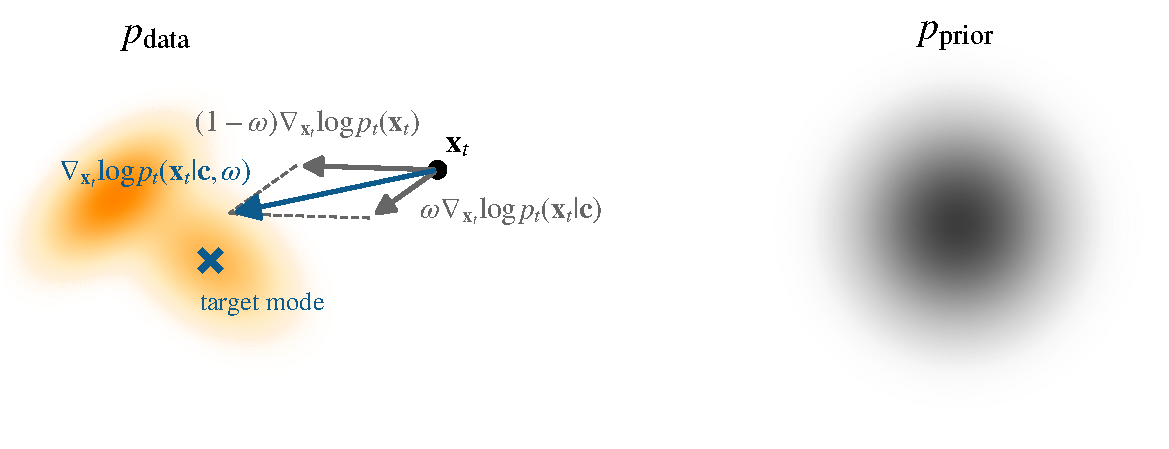
\includegraphics[width=\linewidth]{Images/PartB/classifier_guidance_v2.pdf}
    \caption{\textbfs{CFG 的示意图。} 调整后的分数 $\nabla_{\rvx_t} \log p_t(\rvx_t| \rvc, \omega)$ 由无条件分数 $\nabla_{\rvx_t} \log p_t(\rvx_t)$ 和条件分数 $\nabla_{\rvx_t} \log p_t(\rvx_t| \rvc)$ 之间的线性插值得到，并以 $\omega$ 为权重。所得方向将样本从先验引向与目标条件一致的数据分布模式。 \figcredit{由作者绘制。}}
    \label{fig:cfg}
\end{figure}

\emph{无分类器引导}（CFG）~\citep{ho2021classifier} 是基于分类器引导的一种简化方法，它消除了对独立分类器的需求。其核心思想是以一种无需显式分类器即可实现有效条件化的方式修改分数函数的梯度。具体而言，条件分布对数概率的梯度被调整为如下形式：
\begin{align}
    \nabla_{\rvx_t} \log p_t(\rvc | \rvx_t) = \nabla_{\rvx_t} \log p_t(\rvx_t | \rvc) - \nabla_{\rvx_t} \log p_t(\rvx_t).
\end{align}
将此表达式代入 \Cref{eq:cg_omega}，得到如下条件分数的公式：
\begin{align}\label{eq:cfg-model}
\nabla_{\rvx_t} \log p_t(\rvx_t | \rvc, \omega)
&= \nabla_{\rvx_t} \log p_t(\rvx_t) + \omega \left( \nabla_{\rvx_t} \log p_t(\rvx_t | \rvc) - \nabla_{\rvx_t} \log p_t(\rvx_t) \right) \nonumber\\
&= \omega \underbrace{\nabla_{\rvx_t} \log p_t(\rvx_t | \rvc)}_{\text{条件分数}} + (1 - \omega) \underbrace{\nabla_{\rvx_t} \log p_t(\rvx_t)}_{\text{无条件分数}}.
\end{align}

超参数 $\omega$ 再次在控制条件化信息影响方面发挥关键作用（我们取 $\omega \ge 0$）：
\begin{itemize}
    \item 当 $\omega = 0$ 时，模型表现为无条件扩散模型，完全忽略条件化信息。
    \item 当 $\omega = 1$ 时，模型使用条件分数，没有额外的引导。
    \item 当 $\omega > 1$ 时，模型更加强调条件分数而较少强调无条件分数，增强与 $\rvc$ 的对齐，但通常会降低多样性。
\end{itemize}

\subsection{CFG 的训练与采样}


\paragraph{通过 CFG 联合训练无条件与条件扩散模型。} 与 CG 不同，CFG 需要重新训练一个显式考虑条件变量 $\rvc$ 的扩散模型。然而，为条件和无条件分数函数分别训练两个独立模型通常在计算上不可行。为此，CFG 采用单个模型 $\mathbf{s}_{\bm{\phi}}(\rvx_t, t; \rvc)$，通过将 $\rvc$ 作为额外输入，在单个模型中同时学习两个分数函数。训练过程定义如下：
\begin{itemize}
    \item 对于无条件训练，传入空标记 $\emptyset$ 以替代条件化输入，得到 $\rvs_{\bm{\phi}}(\rvx_t, t, \emptyset)$。
    \item 对于条件训练，提供真实的条件变量 $\rvc$ 作为输入，得到 $\rvs_{\bm{\phi}}(\rvx_t, t, \rvc)$。
\end{itemize}
这两种训练机制通过以概率 $p_\mathrm{uncond}$（一个用户定义的超参数，通常设为 $0.1$）随机将 $\rvc$ 替换为空输入 $\emptyset$ 来统一。这种联合训练策略使模型能够同时学习条件和无条件分数函数。完整的训练算法见 \Cref{alg:cfg_training}，并与 \Cref{alg:no_cfg_training} 中所示的标准无条件训练进行了对比。我们注意到，在训练过程中并不使用 CFG 权重 $\omega$。

\begin{center}
\begin{minipage}[t]{0.48\textwidth}
  \begin{algorithm}[H]
  {\small
    {\small \caption{无条件扩散模型 \label{alg:no_cfg_training} }}
    \begin{algorithmic}[1]
      \Repeat
        \State $\rvx \sim p_{\text{data}}(\rvx)$
        \State $t \sim \mathcal{U}[0, T]$
        \State $\bm{\epsilon} \sim \mathcal{N}(\mathbf{0}, \mathbf{I})$
        \State $\rvx_t = \alpha_t \rvx + \sigma_t \bm{\epsilon}$
        \State 对以下式子进行梯度步：
        \Statex \quad $\nabla_{\bm{\phi}} \left\| \rvs_{\bm{\phi}}(\rvx_t, t) - \rvs \right\|^2$
      \Until{收敛}
    \end{algorithmic}
    }
  \end{algorithm}
\end{minipage}
\hfill
\begin{minipage}[t]{0.48\textwidth}
  \begin{algorithm}[H]
      {\small
    {\small \caption{用于条件扩散模型的 CFG \label{alg:cfg_training}}}
    \begin{algorithmic}[1]
      \Require \textcolor{orange}{$p_\mathrm{uncond}$：无条件 dropout 的概率}
      \Repeat
        \State \textcolor{orange}{$(\rvx, \rvc) \sim p_{\text{data}}(\rvx, \rvc)$}
        \State \textcolor{orange}{以概率 $p_\mathrm{uncond}$ 将 $\rvc \gets \emptyset$}
        \State $t \sim \mathcal{U}[0, T]$
        \State $\bm{\epsilon} \sim \mathcal{N}(\mathbf{0}, \mathbf{I})$
        \State $\rvx_t = \alpha_t \rvx + \sigma_t \bm{\epsilon}$
        \State 对以下式子进行梯度步：
        \Statex \quad \textcolor{orange}{$\nabla_{\bm{\phi}} \left\| \rvs_{\bm{\phi}}(\rvx_t, t, \rvc) - \rvs \right\|^2$}
      \Until{收敛}
    \end{algorithmic}
    }
  \end{algorithm}
\end{minipage}
\end{center}

\paragraph{使用 CFG 进行条件采样。}

一旦使用算法~\ref{alg:cfg_training} 训练了模型 $\rvs_{\bm{\phi}^\times}(\rvx_t, t, \rvc)$，就可以在采样时应用 CFG。对数概率的梯度由下式给出：
\begin{align}\label{eq:cfg-model-nn}
\nabla_{\rvx_t} \log p_t(\rvx_t | \rvc, \omega)
&= \omega \nabla_{\rvx_t} \log p_t(\rvx_t | \rvc) + (1 - \omega) \nabla_{\rvx_t} \log p_t(\rvx_t) \nonumber\\
&\approx \omega \underbrace{\rvs_{\bm{\phi}^\times}(\rvx_t, t, \rvc)}_{\text{条件分数}} + (1 - \omega) \underbrace{\rvs_{\bm{\phi}^\times}(\rvx_t, t, \emptyset)}_{\text{无条件分数}}\\
&=: \rvs_{\bm{\phi}^\times}^{\text{CFG}}(\rvx_t ,t, \rvc; \omega). \nonumber
\end{align}

在采样过程中，应用固定的（或可选地随时间变化的）无分类器引导权重 $\omega$。然后，逆向时间 SDE（\Cref{eq:sde_backward}）或 PF-ODE（\Cref{eq:fp_general}）中的无条件分数 $\nabla_{\rvx_t} \log p_t(\rvx_t)$ 被引导分数 $\rvs_{\bm{\phi}^\times}^{\mathrm{CFG}}(\rvx_t ,t, \rvc; \omega)$ 替换（如 \Cref{eq:condition_prob_ode} 所示），它以加权方式结合了条件分数和无条件分数。

这一公式通过调整 $\omega$ 实现了可控生成，使样本能够在保持多样性的同时被引向条件化信号 $\rvc$。因此，CFG 提供了一种有效且计算高效的方式来实现精确的条件生成，因为它只需训练单个扩散模型。

% \msg{Score Decomposition via Bayes' Rule for Guided Generation}{A key idea behind both CG and CFG is the decomposition of the conditional score into two parts: an unconditional term and a guidance term. This identity follows directly from Bayes' rule (see \Cref{eq:cg_bayes}) and provides a general way to guide diffusion models using auxiliary information. We restate this important formula below, where $\rvy$ denotes the additional information:
% \begin{mdframed}
%     \begin{align}
% \nabla_{\rvx_t} \log p(\rvx_t | \rvy) = \underbrace{\nabla_{\rvx_t} \log p_t(\rvx_t)}_{\text{uncond. direction}}
% + \underbrace{\nabla_{\rvx_t} \log p_t(\rvy | \rvx_t)}_{\text{guidance direction}}. \label{eq:guidance_bayes}
% \end{align}
% \end{mdframed}

% This decomposition makes it possible to use diffusion models in many ways by approximating the guidance term $\nabla_{\rvx_t} \log p_t(\rvy | \rvx_t)$ based on the application. For example, it enables controllable generation by steering samples toward desired attributes $\rvy$, solves inverse problems at test time using observed measurements, and allows one trained model to handle different tasks by applying suitable guidance signals.


% }

\clearpage
\newpage






\section{免训练引导}
本节介绍支撑一大类免训练引导方法~\citep{chung2023diffusion,ye2024tfg,he2024manifold,bansal2023universal} 的高层哲学。尽管在实现和应用上各有差异，这些方法都统一于 \Cref{eq:guidance_bayes} 所表达的核心原则。我们首先在 \Cref{subsec:tfg} 中介绍免训练引导的高层方法，然后将这一思想扩展到免训练的逆问题求解，并在 \Cref{subsec:inverse-problem} 中给出简要概述。


\paragraph{设置与符号。} 设 $\rvc$ 表示条件变量。我们假设可以访问以分数预测表示的预训练扩散模型 $\rvs_{\bm{\phi}^\times}(\rvx_t, t)$\footnote{为简化数学表达，这里我们采用分数和 $\rvx$-预测参数化；其他参数化（例如 $\beps$-预测）可类似处理。}。此外，假设给定一个非负函数
\[
\ell(\cdot, \rvc) \colon \mathbb{R}^D \to \mathbb{R}_{\geq 0}
\]
用于量化样本 $\rvx \in \mathbb{R}^D$ 与条件 $\rvc$ 的对齐程度，其中 $\ell(\rvx, \rvc)$ 的值越小表示对齐越强。此类函数的具体示例包括：(i) $\rvc$ 是参考图像，$\ell(\cdot, \rvc)$ 是度量感知接近度的相似度得分；(ii) $\ell(\cdot, \rvc)$ 是通过预训练模型（例如 CLIP~\citep{radford2021learning}）计算的基于特征的相似度得分。


考虑标准的线性—高斯前向加噪核
 $p_{t}(\cdot| \rvx_0):=\mathcal{N}\big(\cdot; \alpha_t\rvx_0, \sigma^2_t\mathbf{I}\big)$。
我们回顾 \Cref{eq:ddim-update-all} 中的 DDIM 更新，并以它为例：
\begin{align}\label{eq:ddim-update-clean-noise-score}
\begin{aligned}
    \rvx_{t \rightarrow t-1} =\alpha_{t-1} \underbrace{\hat{\rvx}_0(\rvx_t)}_{\text{在数据空间}} - \sigma_{t-1} \sigma_t \underbrace{\hat{\rvs}(\rvx_t)}_{\text{在噪声空间}},
\end{aligned}
\end{align}
其中 $\hat{\rvx}_0(\rvx_t):=\rvx_{\bm{\phi}^\times}(\rvx_t, t)$ 是（干净的）$\rvx$-预测，$\hat{\rvs}(\rvx_t):=\rvs_{\bm{\phi}^\times}(\rvx_t, t)$ 是在时刻水平 $t$ 从 $\rvx_t$ 出发的分数预测。

\subsection{免训练引导的概念框架}\label{subsec:tfg}
大多数免训练引导方法~\citep{ye2024tfg} 在\emph{数据空间}或\emph{噪声空间}中引入校正，以将 \Cref{eq:ddim-update-clean-noise-guide} 中的 DDIM 更新引向满足条件 $\rvc$：
\begin{align}\label{eq:ddim-update-clean-noise-guide}
\begin{aligned}
    \rvx_{t \rightarrow t-1} &=\alpha_{t-1} \underbrace{\left(\hat{\rvx}_0(\rvx_t) + {\color{orange}\eta_t^{\text{data}}\mathcal{G}_0} \right)}_{\text{A. 数据空间}}
    - \sigma_{t-1} \sigma_t \underbrace{\left(\hat{\rvs}(\rvx_t) + {\color{orange}\eta_t^{\text{latent}}\mathcal{G}_t} \right)}_{\text{B. 噪声空间}},
\end{aligned}
\end{align}
其中 $\eta_t^{\text{data}}, \eta_t^{\text{latent}} \geq 0$ 是随时间变化的引导强度，$\mathcal{G}_0$、$\mathcal{G}_t$ 是下面定义的校正项。

\paragraph{A. 数据空间中的引导。}
沿负梯度方向下降
\[
\mathcal{G}_0 := -\nabla_{\rvx_0} \ell(\rvx_0, \rvc),
\]
修改后数据空间中的干净估计
\[
\hat{\rvx}_0(\rvx_t) + {\color{orange}\eta_t^{\text{data}} \mathcal{G}_0},
\]
可以逐步被引向更好地满足条件 $\rvc$ 的样本。这种梯度下降方案可以迭代地应用，以渐进地改善对齐。

代表性示例包括 MGPD~\citep{he2023manifold} 和 UGD~\citep{bansal2023universal}。


% This strategy can also be interpreted as the conditional score decomposition \Cref{eq:guidance_bayes}.

% \begin{align*}
% \nabla_{\rvx_t} \log p_t(\rvx_t|\rvc)
% &= \underbrace{\nabla_{\rvx_t} \log p_t(\rvx_t)}_{\text{unconditional}}
% + \underbrace{\nabla_{\rvx_t} \log p(\rvc|\rvx_t)}_{\text{guidance}}
% \\&\approx \rvs_{\bm{\phi}^\times}(\rvx_t,t) + \eta_t^{\text{latent}} \mathcal{G}_t,
% \end{align*}
% \[
% p(\rvc|\rvx_0) \propto \ell(\rvx_0, \rvc),
% \]
% viewing $\ell_\rvc$ as a surrogate likelihood on the clean signal.

\paragraph{B. 噪声空间中的引导。}
如 \Cref{sec:prologue-guidance} 所讨论，条件分数 $\nabla_{\rvx_t} \log p_t(\rvc|\rvx_t)$ 通常难以处理。一种实用的近似是引入一个替代似然 $\widetilde p_t(\mathbf{c}|\mathbf{x}_t)$：
\[
\widetilde p_t(\mathbf{c}|\mathbf{x}_t) \propto \exp \big(-\eta\ell \left(\hat{\rvx}_0(\rvx_t), \rvc\right)\big)
\]
带有一个重缩放常数 $\eta>0$，使得
\[
\nabla_{\rvx_t}\log \widetilde p_t(\mathbf{c}|\mathbf{x}_t) = -\eta\nabla_{\rvx_t}\ell \left(\hat{\rvx}_0(\rvx_t), \rvc\right) =: \mathcal{G}_t,
\]
其中 $\hat{\rvx}_0(\rvx_t)$ 通过扩散模型的预测得到。
% Then, the guidance direction becomes
% \[
% \nabla_{\rvx_t} \log p_t(\rvc | \rvx_t)
% \approx \nabla_{\rvx_t} \log \ell_\rvc\left(\hat{\rvx}_0(\rvx_t)\right)
% =:\mathcal{G}_t.
% \]
将其代入条件分数的贝叶斯公式，得到代理：
\begin{align*}
\nabla_{\rvx_t} \log p_t(\rvx_t|\rvc)
&\approx \underbrace{\nabla_{\rvx_t} \log p_t(\rvx_t)}_{\text{无条件}}
+ \underbrace{\nabla_{\rvx_t} \log \widetilde p_t(\mathbf{c}|\mathbf{x}_t)}_{\text{引导}}
\\&\approx \hat{\rvs}(\rvx_t) + \eta_t^{\text{latent}} \mathcal{G}_t,
\end{align*}
它充当噪声空间中的引导校正项。


然而，我们注意到计算 $\mathcal{G}_t$ 需要通过 $\rvx$-预测进行反向传播，即
\[
\nabla_{\rvx_t} \hat{\rvx}_0(\rvx_t)^\top \cdot
\left.\nabla_{\rvx_0} \log \ell_{\rvc}(\rvx_0)\right|_{\rvx_0 = \hat{\rvx}_0(\rvx_t)},
\]
这在实践中可能带来相当大的计算开销。

代表性示例包括 \citep{yu2023freedom, chung2022diffusion, bansal2023universal}.




\subsection{免训练方法求解逆问题的示例}\label{subsec:inverse-problem}
\Cref{subsec:tfg} 中介绍的原则在逆问题中有重要的应用。我们先概述背景，然后给出若干具体示例，说明如何利用预训练的扩散模型在推理时求解逆问题。

\paragraph{逆问题的背景。}
设 $\mathcal{A}$ 为退化算子（可以是线性或非线性的，已知或未知的），例如模糊核或图像修复算子，$\mathbf{y}$ 是由如下退化模型生成的观测：
\begin{align}\label{eq:inverse_problem}
    \mathbf{y} = \mathcal{A}(\mathbf{x}_0) + \sigma_{\mathbf{y}} \mathbf{z}, \quad \mathbf{z} \sim \mathcal{N}(\mathbf{0}, \mathbf{I}).
\end{align}
逆问题的目标是从后验分布 $p_0(\mathbf{x}_0 | \mathbf{y})$ 中采样，其中对于给定的观测 $\mathbf{y}$，可能存在无穷多个可能的重建 $\mathbf{x}_0$。目标是恢复一个去除 $\mathbf{y}$ 中退化同时保留其忠实和语义特征的 $\mathbf{x}_0$。


求解逆问题的传统方法通常遵循有监督的框架，需要收集退化样本与恢复样本的成对数据 $(\mathbf{y}, \mathbf{x})$，并依赖优化方法或神经网络的有监督训练。这类方法在数据准备上成本高昂，且对未见数据的泛化能力可能不足。


\paragraph{将预训练扩散模型用作逆问题求解器。}
如前所述，条件分数可以通过贝叶斯法则分解：
\begin{align}
 \nabla_{\rvx_t} \log p_t(\rvx_t | \rvy) = \underbrace{\nabla_{\rvx_t} \log p_t(\rvx_t)}_{\text{数据分数}} + \underbrace{\nabla_{\rvx_t}\log p_t(\rvy | \rvx_t)}_{\text{观测对齐}}.
\label{eq:bayes_rule}
\end{align}

这一分解将数据分数与一个逆问题特有的与 $\rvy$ 的观测对齐项分开。它使我们可以通过对干净数据分布 $ p_{\text{data}} $ 建模并在反演过程中加以应用，从而以无监督方式求解 \Cref{eq:inverse_problem}。更具体地：
\begin{itemize}
    \item \textbfs{数据分数 $\nabla_{\rvx_t} \log p_t(\rvx_t)$：} 使用在干净数据上训练的预训练扩散模型 $\rvs_{\bm{\phi}^\times}(\rvx_t, t)$ 来近似。
    \item \textbfs{观测对齐 $\nabla_{\rvx_t} \log p_t(\rvy | \rvx_t)$：} 没有闭式形式，因为它涉及对隐变量的边缘化。
\end{itemize}

因此，使用预训练扩散模型的大多数免训练方法都聚焦于近似 $\nabla_{\rvx_t} \log p_t(\rvy | \rvx_t)$。我们采用 \citep{daras2024survey} 中总结的一种通用元形式：
\begin{equation*}
    \nabla_{\rvx_t} \log p_t(\rvy | \rvx_t) \approx - \frac{\eqnmarkbox[Plum]{proj}{\mathcal{P}_t}  \, \eqnmarkbox[NavyBlue]{merror}{    \mathcal{M}_t    }}{\eqnmarkbox[OliveGreen]{guidance}{  \gamma_t  }}.
\end{equation*}
其中：
\begin{itemize}
    \item $\mathcal{M}_t$：量化观测 $\rvy$ 与估计信号之间失配的误差向量，
    \item $\mathcal{P}_t$：将 $\mathcal{M}_t$ 投影回 $\rvx_t$ 所处空间的映射，
    \item $\gamma_t$：控制引导强度的标量。
\end{itemize}

代表性方法对 $\mathcal{M}_t$、$\mathcal{P}_t$ 和 $\gamma_t$ 的实例化各不相同，下面以带颜色标注的组件加以说明。

\paragraph{基于扩散模型的逆问题求解器的实例化。}
我们介绍一些代表性方法，它们利用预训练的扩散模型提供无监督方法（无需成对数据），可灵活应用于各种逆问题，且使用同一个学习得到的 $ p_{\mathrm{data}} $ 代理。


\subparagraph{Score SDE~\citep{song2020score}。} 最早基于扩散模型的逆问题求解器之一。它考虑已知的线性退化模型 $\rmA$，并聚焦于 $\sigma_{\rvy} = 0$ 的无噪声设定。由于 $\rmA$ 是线性的，可以构造噪声水平匹配的观测
\[
\rvy_t := \alpha_t \rvy + \sigma_t \bm{\epsilon},
\]
并利用残差 $\rvy_t - \rmA \rvx_t$（注意：一般而言 $\rvy_t \neq \rmA\rvx_t$）驱动一种似然式的校正。一种常见的近似（舍去乘性常数）是
\begin{align*}
    \nabla_{\rvx_t} \log p_t(\rvy|\rvx_t) \approx - \eqnmarkbox[Plum]{proj}{\rmA^\top} (\eqnmarkbox[NavyBlue]{noisymeasurements}{\rvy_t - \rmA \rvx_t}).
\end{align*}

\subparagraph{迭代隐变量细化（ILVR）~\citep{choi2021ilvr}。} 使用与 ScoreSDE 相同的设定，ILVR 估计：
\begin{align*}
    \nabla_{\rvx_t} \log p_t(\rvy| \rvx_t) \approx -\rmA^\dagger(\rvy_t - \rmA\rvx_t) = -\eqnmarkbox[Plum]{moore}{(\rmA^\top \rmA)^{-1} \rmA^\top} (\eqnmarkbox[NavyBlue]{merror}{\rvy_t - \rmA\rvx_t}),
\end{align*}
其中 $\rmA^\dagger$ 是 Moore–Penrose 伪逆，$\rvy_t = \alpha_t\rvy + \sigma_t \bm{\epsilon}_t$。
\subparagraph{扩散后验采样（DPS）~\citep{chung2022diffusion}。} 一种针对已知非线性前向算子 $\mathcal{A}$ 和加性高斯噪声水平 $\sigma_{\rvy} \ge 0$ 的逆问题被广泛使用的方法是\emph{去噪后验分数}（DPS），它近似
\begin{align}\label{eq:dps-score}
  \nabla_{\rvx_t} \log p_t(\rvy|\rvx_t)
   \approx
  \nabla_{\rvx_t} \log p_t\bigl(\rvy|X_0 = \hat\rvx_0(\rvx_t)\bigr),
\end{align}
其中 $\hat\rvx_0(\rvx_t) := \E[\rvx_0|\rvx_t]$ 表示在时刻 $t$ 给定带噪观测 $\rvx_t$ 时干净样本的条件均值，通常用预训练扩散模型通过 Tweedie 公式（\Cref{eq:tweedie}）估计。

这一单点近似假设条件分布 $p(\rvx_0|\rvx_t)$ 高度集中，它源自：
\begin{align*}
  p_t(\rvy|\rvx_t)
  &= \int p_t(\rvy|\rvx_t, \rvx_0)  p(\rvx_0|\rvx_t)  \mathrm{d}\rvx_0 \\
  &= \int p_t(\rvy|\rvx_0)  p(\rvx_0|\rvx_t)  \mathrm{d}\rvx_0
   \approx  p_t\bigl(\rvy|X_0=\hat\rvx_0(\rvx_t)\bigr),
\end{align*}
其中我们利用了在给定 $\rvx_0$ 时 $\rvy$ 仅依赖于 $\rvx_0$（不依赖于 $\rvx_t$）这一事实，且近似在后验 $p(\rvx_0|\rvx_t)$ 紧密集中于其均值的假设下成立。

由于
\[
  p_t\bigl(\rvy|X_0 = \hat\rvx_0(\rvx_t)\bigr)
  = \mathcal{N}\bigl(\rvy;  \mathcal{A}(\hat\rvx_0(\rvx_t)),  \sigma_{\rvy}^2 \rmI\bigr),
\]
我们计算
\begin{align*}
  \nabla_{\rvx_t} \log p_t(\rvy|\rvx_t)
  &\approx \nabla_{\rvx_t} \log \mathcal{N}\bigl(\rvy;  \mathcal{A}(\hat\rvx_0),  \sigma_{\rvy}^2 \rmI\bigr) \\
  &= -\frac{1}{2\sigma_{\rvy}^2}  \nabla_{\rvx_t} \bigl\| \rvy - \mathcal{A}(\hat\rvx_0) \bigr\|^2 \quad  \\
  &= \frac{1}{\sigma_{\rvy}^2}  \left[ \mathcal{J}_{\mathcal{A}}\big(\hat\rvx_0(\rvx_t)\big) \cdot \nabla_{\rvx_t} \hat\rvx_0(\rvx_t) \right]^\top \bigl( \rvy - \mathcal{A}\big(\hat\rvx_0(\rvx_t)\big) \bigr),
\end{align*}
其中 $\mathcal{J}_{\mathcal{A}}\big(\hat\rvx_0(\rvx_t)\big) := \nabla_{\rvx_0} \mathcal{A}(\rvx) \big|_{\rvx = \hat\rvx_0(\rvx_t)}$ 表示前向算子关于其输入的雅可比矩阵。这一公式将梯度通过分数近似流程传播，反映了测量似然如何随带噪样本 $\rvx_t$ 的扰动而变化。

对于线性逆问题，这进一步简化为：
\begin{align*}
    \nabla_{\rvx_t} \log p_t(\rvy | \rvx_t) \approx \eqnmarkbox[OliveGreen]{guidance}{\frac{1}{\sigma_{\rvy}^2}}  \,  \eqnmarkbox[Plum]{proj}{\left[ \rmA \cdot \nabla_{\rvx_t} \hat\rvx_0(\rvx_t) \right]^\top} \left(\eqnmarkbox[NavyBlue]{merror}{\rvy - \rmA(\hat\rvx_0(\rvx_t))}\right).
\end{align*}

大量工作通过为 $\nabla_{\rvx_t} \log p_t(\rvy | \rvx_t)$ 提出各种近似来探索基于扩散模型的逆问题求解器。如需全面综述，读者可参阅 \citet{daras2024survey} 的综述。



\paragraph{一个相关的有监督迭代恢复视角及其与 PF-ODE 的联系。}
上面的讨论通过将预训练扩散先验与 \Cref{eq:bayes_rule} 中的贝叶斯法则分解相结合来求解逆问题。更具体地，这些方法使用先验分布的分数结合测量模型来引导重建过程。同时，它们也反映了一个更广泛的思想：与其一步恢复干净信号，不如通过许多小的更新逐步改进一个退化的输入。类似的高层策略也出现在有监督的图像恢复中，但出发点不同。这些方法不使用预训练的分数模型作为先验，而是直接从成对的退化和干净样本中学习细化过程。

一个代表性示例是 InDI~\citep{delbracio2023inversion}。与上面基于贝叶斯法则的方法不同，InDI 从成对数据 $(\rvy,\rvx_0)$ 出发，其中 $\rvy$ 是退化观测，$\rvx_0$ 是对应的干净目标。重要的是，它一般不假设从 $\rvx_0$ 到 $\rvy$ 的退化过程是解析已知的，也不假设它是高斯的。

其基本思想是通过插值路径连接两个端点
\[
\rvx_t=(1-t)\rvx_0+t\rvy,\qquad t\in[0,1].
\]
这条路径应仅被理解为从干净目标到退化观测的一条方便轨迹。它一般不是高斯加噪过程。沿此路径，对于任意 $0\le s\le t$，有精确关系
\[
\rvx_s=\Bigl(1-\frac{s}{t}\Bigr)\rvx_0+\frac{s}{t}\rvx_t.
\]
对 $\rvx_t$ 取条件期望得到
\[
\mathbb E[\rvx_s|\rvx_t]
=
\Bigl(1-\frac{s}{t}\Bigr)\mathbb E[\rvx_0|\rvx_t]
+
\frac{s}{t}\rvx_t.
\]
这表明，要从当前状态 $\rvx_t$ 移动到一个略微不那么退化的状态，只需从 $\rvx_t$ 预测干净目标即可。

基于这一思想，人们从成对样本中通过最小化回归目标训练一个时间条件预测器 $\rmF_{\bphi}(\rvx_t,t)$
\[
\min_{\bphi}\;
\mathbb E_{(\rvx_0,\rvy)\sim p(\rvx_0,\rvy),\, t\sim p(t)}
\Bigl\|
\rmF_{\bphi}\bigl((1-t)\rvx_0+t\rvy,\,t\bigr)-\rvx_0
\Bigr\|_2^2,
\]
其中 $p(\rvx_0,\rvy)$ 表示由干净目标 $\rvx_0$ 及其退化观测 $\rvy$ 组成的数据对的联合分布，$p(t)$ 指定训练时插值时间如何采样。
也就是说，$\rmF_{\bphi}$ 被训练为从沿插值路径的中间退化状态预测干净目标。对于这一平方误差损失，贝叶斯最优预测器是条件期望
\[
\rmF^*(\rvx_t,t)=\mathbb E[\rvx_0|\rvx_t].
\]
因此，如果模型类足够有表达力且优化成功，学习得到的预测器近似于时刻 $t$ 与中间状态 $\rvx_t$ 关联的平均干净目标。在这个意义上，训练目标在精神上类似于扩散模型的训练：两者都是学习一个从中间退化状态到更干净目标的时间条件回归。区别在于扩散模型从规定的前向退化过程中合成地生成这样的训练对，而这里的端点对 $(\rvy,\rvx_0)$ 直接来自有监督的恢复数据。

在推理时，从 $\hat{\rvx}_1=\rvy$ 开始，反复通过下式细化估计
\[
\hat{\rvx}_{t-\Delta t}
=
\frac{\Delta t}{t}\rmF_{\bphi}(\hat{\rvx}_t,t)
+
\Bigl(1-\frac{\Delta t}{t}\Bigr)\hat{\rvx}_t.
\]
因此，最终重建是由逐步细化而非单次直接预测产生的。在连续时间极限下，这导出 InDI 的残差流 ODE
\[
\frac{\diff \rvx_t}{\diff t}
=
\frac{\rvx_t-\rmF_{\bphi}(\rvx_t,t)}{t}.
\]

现在假设我们进一步特化到高斯去噪设定，即假设退化取已知的解析形式
\[
\rvy=\rvx_0+\sigma\beps,
\qquad \beps\sim\mathcal N(\bm 0,\rmI),
\]
噪声水平 \(\sigma\) 已知。在这一特化下，InDI 的残差流 ODE 恰好退化为概率流 ODE。事实上，插值路径变为
\[
\rvx_t=(1-t)\rvx_0+t\rvy
=
\rvx_0+t\sigma\beps,
\]
这正是标准扩散形式
\[
\rvx_t=\alpha_t\rvx_0+\sigma_t\beps,
\qquad\text{其中}\qquad
\alpha_t=1,\;\sigma_t=t\sigma.
\]
因此，预测器 \(\rmF_{\bphi}(\rvx_t,t)\approx \mathbb E[\rvx_0\mid \rvx_t]\) 现在学习的是对高斯退化的中间状态 \(\rvx_t\) 进行去噪。此时，残差流 ODE 变为
\[
\frac{\diff \rvx_t}{\diff t}
=
\frac{\rvx_t-\mathbb E[\rvx_0\mid \rvx_t]}{t}
=
-\dot{\sigma}_t\sigma_t\nabla_{\rvx_t}\log p_t(\rvx_t),
\]
其中最后一个等式由 \(\sigma_t=t\sigma\) 以及 Tweedie 公式得到，
\[
\mathbb E[\rvx_0\mid \rvx_t]
=
\rvx_t+\sigma_t^2\nabla_{\rvx_t}\log p_t(\rvx_t).
\]
这正是该高斯去噪路径的 PF-ODE，写成去噪器形式或分数形式。因此，在高斯去噪特化下，InDI 给出了扩散建模的另一种解释：可以将其视为在高斯退化数据上的有监督去噪器学习，而 PF-ODE 作为逐步细化的连续时间极限出现。



\newpage
\section{从强化学习到用于模型对齐的直接偏好优化}\label{sec:rlhf-dpo}

% In the pursuit of aligning generative models with human intent, the prevailing paradigm has been Reinforcement Learning from Human Feedback (RLHF). While effective, RLHF is a complex, multi-stage process prone to instability. This section introduces \emph{Direct Preference Optimization (DPO)}, a more streamlined and stable method that achieves the same objective without the need for explicit reward modeling or reinforcement learning. We then explore its extension to a different generative class with \emph{Diffusion-DPO}.

% \subsection{The Motivation: Circumventing the Pitfalls of RLHF}

% The goal of alignment is to steer a base, pre-trained model (such as a supervised fine-tuned LLM) to produce outputs that humans prefer. The RLHF framework tackles this in three distinct stages. First, supervised fine-tuning (SFT) trains a base model on a dataset of prompt-response pairs. Second, reward modeling (RM) trains a separate model on human preferences consisting of prompts $\mathbf{c}$ and paired responses, one preferred ($\mathbf{x}_w$, ``winner'') and one dispreferred ($\mathbf{x}_l$, ``loser''), with the reward model $r(\mathbf{c},\mathbf{x})$ assigning higher scalar reward to the winner. Finally, RL fine-tuning optimizes the SFT model (now a policy $\pi$) using an RL algorithm such as PPO, maximizing reward-model scores while being regularized by a KL-divergence penalty that keeps $\pi$ close to the reference distribution.

% Despite its impact, this pipeline suffers from drawbacks: the RL stage is unstable and computationally expensive, involving repeated sampling from the policy; it requires training and hosting multiple large models (SFT, reward, and possibly value models); and it optimizes only a proxy for human preferences, meaning flaws in the reward model can be exploited. This motivates a central question:
% \begin{question}
%     Can we eliminate explicit reward modeling and the unstable RL process, directly optimizing the model on preference data?
% \end{question}
在追求将生成式模型与人类意图对齐的过程中，主流范式一直是基于人类反馈的强化学习（RLHF）。尽管有效，RLHF 是一个复杂、多阶段且可能不稳定的过程。本节介绍\emph{直接偏好优化（DPO）}~\citep{rafailov2023direct}，它是一种更精简且稳定的方法，无需显式奖励建模或强化学习即可达到同样的目标。随后我们概述它通过 \emph{Diffusion-DPO}~\citep{wallace2024diffusion} 向扩散模型的扩展。

\subsection{动机：规避 RLHF 的陷阱}

对齐的目标是将一个基础的预训练模型（例如 SFT 模型）引导向人类偏好的输出。RLHF 分三个阶段进行。首先，\emph{有监督微调（SFT）}在提示—响应对上训练一个基础模型。其次，\emph{奖励建模（RM）}在偏好数据上拟合一个模型，该数据由提示 $\mathbf{c}$ 和成对的响应（一个偏好的"赢家" $\mathbf{x}_w$ 和一个不偏好的"输家" $\mathbf{x}_l$）组成，学习一个标量 $r(\mathbf{c},\mathbf{x})$ 使得 $r(\mathbf{c},\mathbf{x}_w)>r(\mathbf{c},\mathbf{x}_l)$。第三，\emph{RL 微调}用诸如 PPO~\citep{schulman2017proximal} 之类的算法优化 SFT 模型（策略 $\pi$\footnote{策略将一个提示/历史（状态）映射到响应/动作上的分布。}），最大化来自 $r$ 的期望奖励，同时通过 KL 惩罚进行正则化，使 $\pi$ 保持在参考/SFT 分布附近。

尽管影响深远，这一流程存在缺陷：RL 阶段不稳定且计算昂贵，因为它是同策略的——每次更新都需要从当前模型新鲜生成的样本；它还需要训练和部署多个大型模型（SFT、奖励，有时还有价值模型）；而且它只优化人类偏好的代理，因此奖励模型中的缺陷可能被利用。这引出一个核心问题：
\begin{question}
    我们能否消除显式的奖励建模和不稳定的 RL 步骤，直接在偏好数据上优化模型？
\end{question}

直接偏好优化（DPO）通过用单个、有监督式的步骤替代多阶段的 RLHF 流程来简化对齐。DPO 不再训练一个单独的奖励模型并运行像 PPO 这样不稳定的 RL 算法，而是直接用一个简单的逻辑损失将策略拟合到偏好对上，同时保持接近一个固定的参考模型。其关键洞察是，KL 正则化的 RLHF 目标可以被改写，使得策略与参考之间的对数似然比充当一个隐式奖励。这保留了对参考策略的相同正则化，但避免了昂贵的采样回放和显式奖励建模。

在 \Cref{subsec:rlhf-bradley-terry} 中，我们简要回顾 RLHF 流程及其对大型奖励模型和 RL 微调的依赖。在 \Cref{subsec:dpo} 中，我们介绍最初为语言模型提出的 DPO，它规避了奖励模型训练并简化了对齐微调。最后，在 \Cref{subsec:diffusion-dpo} 中，我们将这一思想扩展到扩散模型，把 Diffusion-DPO 作为生成式建模场景中一种实用且稳定的对齐方法加以介绍。

\subsection{RLHF：Bradley--Terry 视角}\label{subsec:rlhf-bradley-terry}


\paragraph{RLHF 简要介绍。}
RLHF 从一个学习得到的评判者开始：一个奖励模型 $r_{\bm\psi}$，它为同一提示 $\mathbf c$ 的候选响应赋予标量偏好分数。数据集 $\mathcal D$ 由成对的 $(\tilde{\mathbf x},\mathbf x)$ 组成，并标注了标签 $y$，指示 $\tilde{\mathbf x}$ 是否优于 $\mathbf x$。标签可以是二值的 $y\in\{0,1\}$，也可以是通过汇总多个评分者得到的软值 $y\in[0,1]$。训练目标是一个简单的逻辑损失
\begin{align}\label{eq:rm-emp}
\begin{aligned}
    \mathcal L_{\mathrm{RM}}(\bm\psi)
=
- \mathbb E_{(\mathbf c,\tilde{\mathbf x},\mathbf x,y)\sim\mathcal D}
\Big[
y &\log \sigma \big(r_{\bm\psi}(\mathbf c,\tilde{\mathbf x})-r_{\bm\psi}(\mathbf c,\mathbf x)\big)
\\ &+(1-y)\log \big(1-\sigma \big(r_{\bm\psi}(\mathbf c,\tilde{\mathbf x})-r_{\bm\psi}(\mathbf c,\mathbf x)\big)\big)
\Big],
\end{aligned}
\end{align}
其中 $\sigma(u)=1/(1+e^{-u})$。在实践中，$\mathcal D$ 中的偏好对可能来自多种来源：精选的响应、不同检查点处的模型快照，或预训练条件扩散模型的生成结果。
一种标准约定是以有序格式 $(\text{赢家}, \text{输家})$ 存储它们。
在这一约定下，我们简单地设 $y=1$，\Cref{eq:rm-emp} 退化为特例（令 $\tilde\rvx = \rvx^w$ 且 $\rvx = \rvx^l$）：
\begin{equation}\label{eq:rm-bt}
\mathcal L_{\mathrm{RM}}(\bm\psi)
=
- \mathbb E_{(\mathbf c,\mathbf x_w,\mathbf x_l)\sim\mathcal D}
\Big[\log \sigma \big(r_{\bm\psi}(\mathbf c,\mathbf x_w)-r_{\bm\psi}(\mathbf c,\mathbf x_l)\big)\Big].
\end{equation}


\paragraph{Bradley--Terry 视角与 KL 联系。}
通常通过 Bradley--Terry（BT）模型~\citep{bradley1952rank} 来解释
\[
p_{r_{\bm\psi}}(\tilde{\mathbf x}\succ \mathbf x|\mathbf c)
 := \sigma \big(r_{\bm\psi}(\mathbf c,\tilde{\mathbf x})-r_{\bm\psi}(\mathbf c,\mathbf x)\big)
\]
该模型将两个标量分数转换为获胜概率。
这一表述突出了两个关键性质：(i) 只有分数的\emph{差}才重要（因此 $r_{\bm\psi}(\mathbf c,\cdot)$ 是平移不变的），(ii) 损失推动预测赢家的分数高于输家的分数。为了直观理解 (ii)，考虑一个标签为 $y\in\{0,1\}$ 的对，并定义
\[
\Delta r := r_{\bm\psi}(\mathbf c,\tilde{\mathbf x})-r_{\bm\psi}(\mathbf c,\mathbf x),
\quad
p:=\sigma(\Delta r),\quad \sigma(u)=\tfrac{1}{1+e^{-u}}.
\]
单样本的逻辑损失是
\[
\ell=-\big[y\log p+(1-y)\log(1-p)\big].
\]
那么
\[
\frac{\partial \ell}{\partial \Delta r}=\sigma(\Delta r)-y.
\]
在步长 $\eta>0$ 的梯度下降下，分数差的更新为
\[
\Delta r \leftarrow \Delta r-\eta\big(\sigma(\Delta r)-y\big).
\]
因此，如果 $y=1$（"$\tilde{\mathbf x}$ 获胜"），则 $\sigma(\Delta r)-1\le 0$，所以 $\Delta r$ 增大（赢家升、输家降）；如果 $y=0$，则 $\Delta r$ 减小。


\Cref{eq:rm-emp} 中的每个单样本项可以视为观测到的伯努利标签与模型预测的获胜概率之间的交叉熵：
\[
-\big[y\log p_{r_{\bm\psi}}+(1-y)\log(1-p_{r_{\bm\psi}})\big]
= \mathcal D_{\mathrm{KL}} \big(\mathrm{Bern}(y) \big\| \mathrm{Bern}(p_{r_{\bm\psi}})\big)
+ \mathcal H \big(\mathrm{Bern}(y)\big),
\]
其中 $\mathcal H$ 是目标伯努利分布的熵。
在数据集 $\mathcal D$ 上平均得到
\begin{align}\label{eq:reward_loss}
    \mathcal L_{\mathrm{RM}}(\bm\psi)
= \mathbb E_{\mathcal D} \Big[\mathcal D_{\mathrm{KL}}\left(\mathrm{Bern}(y) \big\| \mathrm{Bern}(p_{r_{\bm\psi}})\right)\Big]
+ \underbrace{\mathbb E_{\mathcal D} \big[\mathcal H(\mathrm{Bern}(y))\big]}_{\text{与 }\bm\psi 无关}.
\end{align}
因此，最小化逻辑损失等价于最小化人类标签的经验伯努利分布与模型预测的伯努利分布之间的 KL 散度。在二值情形（$y\in\{0,1\}$）下，这一等价是精确的；对于软标签（$y\in[0,1]$），结果在差一个熵常数偏移的意义下成立。直观地说，奖励模型被训练为调整其获胜概率，直到它们与数据集中观测到的经验人类获胜率相一致。

从这一点起，我们采用最常见的约定：$\mathcal D$ 以有序格式存储成对数据：$(\rvx^w, \rvx^l, \rvc) \sim \mathcal D$。在这一约定下，标签总是 $y=1$，损失简化为 \Cref{eq:rm-bt} 中给出的有序形式，我们将在下面的讨论中使用它。

\paragraph{KL 正则化的策略优化（固定奖励）。}
用通过 \Cref{eq:rm-bt} 训练得到的奖励 $r:=r_{\bm\psi^\times}$，以及条件预训练扩散模型 $p_{\bm{\phi}^\times}(\mathbf x|\mathbf c)$，RLHF 随后调整一个可学习的策略 $\pi_{\bm\theta}(\mathbf x|\mathbf c)$（通常在 $p_{\bm{\phi}^\times}(\mathbf x|\mathbf c)$ 之上微调），使其朝向更高奖励的响应。
同时，策略通过 $\mathcal{D}_{\mathrm{KL}}$ 惩罚被正则化以保持接近一个参考模型，该参考模型取为预训练扩散模型 $\pi_{\mathrm{ref}}(\mathbf x|\mathbf c):=p_{\bm{\phi}^\times}(\mathbf x|\mathbf c)$：
\begin{equation}\label{eq:rlhf-policy-correct}
\max_{\bm\theta}
\mathbb E_{\mathbf c\sim p(\mathbf c)}
\Big[
\mathbb E_{\mathbf x\sim \pi_{\bm\theta}(\cdot|\mathbf c)}\big[r_{\bm\psi}(\mathbf c,\mathbf x)\big]
-\beta \mathcal{D}_{\mathrm{KL}} \big(\pi_{\bm\theta}(\cdot|\mathbf c) \big\| \pi_{\mathrm{ref}}(\cdot|\mathbf c)\big)
\Big],
\end{equation}
它使两种力量变得显式：寻找评判者偏好的样本，但保持接近预训练参考。

我们注意到 \Cref{eq:rm-bt} 中的奖励目标仅使用带标签的对，且不要求 $\mathcal D$ 由参考模型（即预训练条件扩散模型）生成。虽然不是必需的，但从接近目标策略的模型中收集对可以减少分布偏移，并使所学到的奖励在它将要使用的区域更可靠。

总之，RLHF 分两个阶段进行：首先通过最小化 \Cref{eq:rm-bt} 中的损失（等价于 \Cref{eq:reward_loss} 中的期望二值 $\mathcal{D}_{\mathrm{KL}}$）来拟合奖励 $r^*$；然后通过求解 \Cref{eq:rlhf-policy-correct} 来优化策略 $\pi^*$。


\newpage


% \paragraph{Short Introduction to RLHF.}
% RLHF starts with a learned judge: a reward model $r_{\bm\psi}$ that predicts which of two candidates better matches human preferences. For each prompt $\mathbf c$ we observe a pair $(\mathbf x_w,\mathbf x_l)$ where humans prefer the former. The practical training objective on a dataset $\mathcal D$ of labeled pairs is the sample average
% \begin{equation}\label{eq:rm-emp}
% {\mathcal L}_{\mathrm{RM}}(\bm\psi)
% =
% - \mathbb E_{(\mathbf c,\mathbf x_w,\mathbf x_l)\sim\mathcal D}
% \Big[\log \sigma \big(r_{\bm\psi}(\mathbf c,\mathbf x_w)-r_{\bm\psi}(\mathbf c,\mathbf x_l)\big)\Big],
% \end{equation}
% where $\sigma(u)=1/(1+e^{-u})$. It is standard to interpret the score difference through the Bradley--Terry (BT) model, which maps scores to a win probability
% \[
% p_r(\tilde{\mathbf x}\succ \mathbf x|\mathbf c)
% := \sigma \big(r_{\bm\psi}(\mathbf c,\tilde{\mathbf x})-r_{\bm\psi}(\mathbf c,\mathbf x)\big).
% \]
% This view explains shift invariance of $r_{\bm\psi}(\mathbf c,\cdot)$. In practice, pairs in $\mathcal D$ may come from any pool (curated responses, different checkpoints, baselines) and could be mixed; one can imagine a simple special case where they were proposed by a fixed conditional generator (such as a pre-trained fixed conditional diffusion model $p_{\bm{\phi}^\times}(\mathbf x|\mathbf c)$), but this is not necessary.

% \paragraph{Equivalence to KL minimization.}
% Let $p_{\mathrm{tgt}}(\mathbf c,\mathbf x,\tilde{\mathbf x})$ denote the (oracle or population) distribution that describes how prompts and candidate pairs are drawn, and let
% $p_{\mathrm{gt}}(\tilde{\mathbf x}\succ \mathbf x|\mathbf c)\in[0,1]$ be the (unknown) human win probability for that pair. The corresponding oracle (population) objective integrates over the random human vote:
% \begin{align}\label{eq:rm-pop}
% \begin{aligned}
%     \mathcal L_{\mathrm{RM}}(\bm\psi)
% = - \mathbb E_{(\mathbf c,\mathbf x,\tilde{\mathbf x})\sim p_{\mathrm{tgt}}}
% \Big[
% & p_{\mathrm{gt}}(\tilde{\mathbf x}\succ \mathbf x|\mathbf c) \log p_r(\tilde{\mathbf x}\succ \mathbf x|\mathbf c) \\
% &+ \big(1-p_{\mathrm{gt}}(\tilde{\mathbf x}\succ \mathbf x|\mathbf c)\big) \log \big(1-p_r(\tilde{\mathbf x}\succ \mathbf x|\mathbf c)\big)
% \Big].
% \end{aligned}
% \end{align}
% This is the cross entropy between $p_{\mathrm{gt}}:=p_{\mathrm{gt}}(\tilde{\mathbf x}\succ \mathbf x|\mathbf c)$ and the BT probability
% $p_r:=p_r(\tilde{\mathbf x}\succ \mathbf x|\mathbf c)$.

% Since  the cross-entropy of $p_{\mathrm{gt}}$ and $p_r$, $\mathrm{CE}(p_{\mathrm{gt}},p_r)$, is related to their KL divergence denotes via
% \begin{align*}
%     \mathrm{CE}(p_{\mathrm{gt}},p_r)&=-p_{\mathrm{gt}}\log p_r-(1-p_{\mathrm{gt}})\log(1-p_r)\\   &=\mathcal{D}_{\mathrm{KL}}(\mathrm{Bern}(p_{\mathrm{gt}}) \| \mathrm{Bern}(p_r))+\mathcal{H}(\mathrm{Bern}(p_{\mathrm{gt}})),
% \end{align*}
% with $\mathrm{Bern}(\cdot)$ denotes the Bernoulli distribution (i.e., binary) and $\mathcal{H}(\cdot)$ denotes the entropy, minimizers of $\mathcal L_{\mathrm{RM}}$ are the same as minimizers of the expected Bernoulli KL:
% \begin{equation}\label{eq:reward_loss}
% \min_{\bm\psi}
% \mathbb E_{(\mathbf c,\mathbf x,\tilde{\mathbf x})\sim p_{\mathrm{tgt}}}
% \big[\mathcal D_{\mathrm{KL}} \big(\mathrm{Bern}(p_{\mathrm{gt}}) \big\| \mathrm{Bern}(p_r)\big)\big].
% \end{equation}
% Connection to the empirical objective: ${\mathcal L}_{\mathrm{RM}}(\bm\psi)$ in \Cref{eq:rm-emp} is a sample approximation to \Cref{eq:rm-pop}. Concretely, replace the expectation over $p_{\mathrm{tgt}}$ by the sample average over $\mathcal D$, and replace the unknown $p_{\mathrm{gt}}$ by the observed label $y$ (or a soft label from multiple raters): for instance each datum is $(\mathbf c,\mathbf x_w,\mathbf x_l)$ with the winner first, the label is implicit ($y=1$). If one adopts a fixed pre-trained model $p_{\bm{\phi}^\times}(\cdot|\rvc)$ to create $p_{\mathrm{tgt}}(\mathbf c,\mathbf x,\tilde{\mathbf x})$, then $p_{\mathrm{tgt}}(\mathbf c,\mathbf x,\tilde{\mathbf x}) = p(\mathbf c) p_{\bm{\phi}^\times}(\mathbf x|\mathbf c) p_{\bm{\phi}^\times}(\tilde{\mathbf x}|\mathbf c)$, but the KL view and the empirical approximation do not rely on this specific choice.

% Therefore minimizing \Cref{eq:rm-pop} is equivalent to minimizing the expected Bernoulli KL, since the entropy term does not depend on $\bm\psi$. In practice we approximate the population objective by the empirical one in \Cref{eq:rm-emp}: replace the population expectation over $p_{\mathrm{tgt}}$ by the sample average over $\mathcal D$, and replace $p_{\mathrm{gt}}$ by the observed label ($y$ or a soft $\hat p$).


% \newpage


% \paragraph{Short Introduction to RLHF.}
% To see where DPO comes from, it helps to view RLHF as beginning with a learned judge: a reward model that scores which of two candidates better matches human preferences. Concretely, for each prompt (context) $\mathbf c$ we observe a pair $(\mathbf x_w,\mathbf x_l)$ where humans prefer the former. Training the judge is just logistic regression on preference pairs:
% \begin{equation}\label{eq:rm-bt}
% \mathcal L_{\mathrm{RM}}(\bm\psi)
% =
% - \mathbb E_{(\mathbf c,\mathbf x_w,\mathbf x_l)\sim\mathcal D}
% \Big[ \log \sigma \big(r_{\bm\psi}(\mathbf c,\mathbf x_w)-r_{\bm\psi}(\mathbf c,\mathbf x_l)\big) \Big],
% \end{equation}
% where $r_{\bm\psi}$ is the reward model and $\sigma(u)=1/(1+e^{-u})$ is the logistic function.
% Equivalently, one can imagine that the dataset $\mathcal D$ arises by first sampling a prompt $\mathbf c\sim p(\mathbf c)$, then drawing two candidates independently from a fixed pre-trained conditional generator $\pi_{\mathrm{ref}}(\cdot|\mathbf c):=p_{\bm{\phi}^\times}(\cdot|\mathbf c)$ (e.g., a pre-trained conditional diffusion model or its SFT fine-tuned version), and finally labeling the pair according to a (possibly stochastic) human preference probability $p_{\mathrm{gt}}(\tilde{\mathbf x}\succ \mathbf x|\mathbf c)\in[0,1]$. The corresponding population loss is the binary cross-entropy
% \begin{align}\label{eq:rm-pop}
% \begin{aligned}
%     \mathcal L_{\mathrm{RM}}(\bm\psi)
% = - \mathbb E_{\substack{\mathbf c\sim p(\mathbf c)\\ \mathbf x,\tilde{\mathbf x}\sim \pi_{\mathrm{ref}}(\cdot|\mathbf c)}}
% \Big[
% & p_{\mathrm{gt}}(\tilde{\mathbf x}\succ \mathbf x|\mathbf c) \log \sigma \big(r_{\bm\psi}(\mathbf c,\tilde{\mathbf x})-r_{\bm\psi}(\mathbf c,\mathbf x)\big) \\
% &+\big(1-p_{\mathrm{gt}}(\tilde{\mathbf x}\succ \mathbf x|\mathbf c)\big) \log \sigma \big(r_{\bm\psi}(\mathbf c,\mathbf x)-r_{\bm\psi}(\mathbf c,\tilde{\mathbf x})\big)
% \Big].
% \end{aligned}
% \end{align}
% This formulation makes the roles explicit: $p(\mathbf c)$ governs prompts, $\pi_{\mathrm{ref}}=p_{\bm{\phi}^\times}$ proposes candidate responses for each prompt, $p_{\mathrm{gt}}$ captures human preference noise, and the reward model $r_{\bm\psi}$ is trained to predict which candidate wins.

% \paragraph{Reward Model Training via Bradley--Terry View.}
% Each comparison yields a binary outcome: “does $\tilde{\mathbf x}$ win over $\mathbf x$ for the same prompt $\mathbf c$?”
% The Bradley--Terry (BT) model~\citep{bradley1952rank} is the simplest, shift-invariant way to convert scalar preference ratings (logits) into pairwise win probabilities: the probability of preferring $\tilde{\mathbf x}$ depends only on the difference of their preference ratings. If the trainable reward $r_{\bm\psi}(\mathbf c,\cdot)$ assigns higher scores to better candidates, BT posits
% \begin{equation*}
% p_r(\tilde{\mathbf x}\succ \mathbf x |\mathbf c)
% = \sigma \big(r_{\bm\psi}(\mathbf c,\tilde{\mathbf x})-r_{\bm\psi}(\mathbf c,\mathbf x)\big),
% \end{equation*}
% so adding any constant to $r_{\bm\psi}$ leaves preferences unchanged.

% Fitting $r_{\bm\psi}$ with \Cref{eq:rm-bt} is exactly maximum likelihood for the BT model on pairwise data.
% To see this, rewrite \Cref{eq:rm-pop} as a cross-entropy between the ``human win rate''
% $p_{\mathrm{gt}}:=p_{\mathrm{gt}}(\tilde{\mathbf x}\succ \mathbf x|\mathbf c)$ and the BT probability
% $p_r:=p_r(\tilde{\mathbf x}\succ \mathbf x|\mathbf c)$:
% \[
% \mathcal L_{\mathrm{RM}}(\bm\psi)
% =\mathbb E_{\substack{\mathbf c\sim p(\mathbf c)\\ \mathbf x,\tilde{\mathbf x}\sim \pi_{\mathrm{ref}}(\cdot|\mathbf c)}}
%  \Big[ \underbrace{-p_{\mathrm{gt}}\log p_r-(1-p_{\mathrm{gt}})\log(1-p_r)}_{\mathrm{CE}(p_{\mathrm{gt}},p_r)} \Big].
% \]
% Here, $\mathrm{CE}(p_{\mathrm{gt}},p_r)$ denotes the cross-entropy of $p_{\mathrm{gt}}$ and $p_r$. Since
% \[
% \mathrm{CE}(p_{\mathrm{gt}},p_r)=\mathcal{D}_{\mathrm{KL}}(\mathrm{Bern}(p_{\mathrm{gt}}) \| \mathrm{Bern}(p_r))+\mathcal{H}(\mathrm{Bern}(p_{\mathrm{gt}})),
% \]
% where $\mathrm{Bern}(\cdot)$ denotes the Bernoulli distribution (i.e., binary) and $\mathcal{H}(\cdot)$ denotes the entropy, minimizers of \Cref{eq:rm-pop} are exactly the minimizers of the expected (Bernoulli) KL:
% \begin{equation}\label{eq:reward_loss}
% \min_{\bm\psi}
% \mathbb E_{\substack{\mathbf c\sim p(\mathbf c)\\ \mathbf x,\tilde{\mathbf x}\sim \pi_{\mathrm{ref}}(\cdot|\mathbf c)}}
% \Big[\mathcal{D}_{\mathrm{KL}}\big(\mathrm{Bern}(p_{\mathrm{gt}}) \big\| \mathrm{Bern}(p_r)\big)\Big],
% \end{equation}
% because $\mathcal{H} \big(\mathrm{Bern}(p_{\mathrm{gt}})\big)$ does not depend on $\bm\psi$.
% In simple words, training the reward model via \Cref{eq:rm-pop} closes the gap between the judge’s opinion ($p_r$) and the human preference ($p_{\mathrm{gt}}$).

% \paragraph{KL Regularized Policy Optimization (with Fixed Reward).}
% With the fitted reward $r:=r_{\bm\psi^\times}$ in hand trained via \Cref{eq:rm-bt}, RLHF then adjusts a learnable policy $\pi_{\bm\theta}(\mathbf x|\mathbf c)$ toward higher-reward responses while keeping it close to a reference $\pi_{\mathrm{ref}}(\mathbf x|\mathbf c):=p_{\bm{\phi}^\times}(\mathbf x|\mathbf c)$ via a $\mathcal{D}_{\mathrm{KL}}$ regularizer:
% \begin{equation}\label{eq:rlhf-policy-correct}
% \max_{\bm\theta}
% \mathbb E_{\mathbf c\sim p(\mathbf c)}
% \Big[
% \mathbb E_{\mathbf x\sim \pi_{\bm\theta}(\cdot|\mathbf c)}\big[r_{\bm\psi}(\mathbf c,\mathbf x)\big]
% -\beta \mathcal{D}_{\mathrm{KL}} \big(\pi_{\bm\theta}(\cdot|\mathbf c) \big\| \pi_{\mathrm{ref}}(\cdot|\mathbf c)\big)
% \Big],
% \end{equation}
% which makes the two forces explicit: seek samples the judge prefers, but stay close to the pre-trained reference.

% \textit{Clarification.} The reward objective in \Cref{eq:rm-emp} uses only labeled pairs and does not require that $\mathcal D$ be generated by the reference model. By contrast, the policy objective \Cref{eq:rlhf-policy-correct} does require a fixed reference $\pi_{\mathrm{ref}}$ (commonly the pre-trained conditional diffusion model), which defines the KL term and usually initializes $\pi_{\bm\theta}$. While not required, collecting pairs from models close to the intended policy can reduce distribution shift and make the learned reward more reliable in the region where it will be used.




% In summary, RLHF proceeds in two stages: first fit the reward $r^*$ by minimizing the population loss in \Cref{eq:rm-pop} (equivalently, the expected binary $\mathcal{D}_{\mathrm{KL}}$ in \Cref{eq:reward_loss}); then optimize the policy $\pi^*$ by solving \Cref{eq:rlhf-policy-correct}.


\subsection{DPO 框架}\label{subsec:dpo}
\paragraph{从 RLHF 出发的桥梁。}
给定拟合的奖励 $r := r_{\bm\psi^\times}$，\Cref{eq:rlhf-policy-correct} 中的 KL 正则化策略目标对每个提示 $\mathbf c$ 都有一个简单的闭式解，表示为如下的基于能量的形式~\citep{peters2010relative}：
\begin{equation}\label{eq:rlhf-closed-form}
\pi^*(\mathbf x|\mathbf c)
=
\frac{1}{Z(\mathbf c)} \pi_{\mathrm{ref}}(\mathbf x|\mathbf c)\exp(r(\mathbf c,\mathbf x)/\beta),
\end{equation}
其中 $\pi_{\mathrm{ref}}(\mathbf x|\mathbf c):=p_{\bm{\phi}^\times}(\mathbf x|\mathbf c)$，$Z(\mathbf c)$ 是保证 $\int \pi^*(\mathbf x|\mathbf c) \diff \mathbf x=1$ 的配分函数。

对于较小的 $\beta$，$\exp(r/\beta)$ 变得更尖锐，因此 $\pi^*$ 集中在高奖励区域：奖励占主导，策略离 $\pi_{\mathrm{ref}}$ 更远，多样性下降，训练可能变得不稳定或容易受到奖励黑客攻击。对于较大的 $\beta$，$\exp(r/\beta)$ 变平，使 $\pi^*$ 更接近 $\pi_{\mathrm{ref}}$：KL 项占主导，更新保守，多样性跟随参考，但奖励增益有限。

由于我们的目标是直接微调策略（不训练单独的奖励模型），\Cref{eq:rlhf-closed-form} 让我们可以从任意策略\emph{定义}一个\textit{隐式奖励}。下面我们引入：
\paragraph{由对 \Cref{eq:rlhf-closed-form} 取逆所启发的隐式奖励定义。}
\Cref{eq:rlhf-closed-form} 提示一种立即的求逆：对任意策略 $\pi$（其支撑包含在 $\pi_{\mathrm{ref}}$ 中），定义
\begin{equation}\label{eq:implicit-reward}
r_{\pi}(\mathbf c,\mathbf x)
 =
\beta \log\frac{\pi(\mathbf x|\mathbf c)}{\pi_{\mathrm{ref}}(\mathbf x|\mathbf c)}
 + \beta \log Z(\mathbf c).
\end{equation}
则 \Cref{eq:rlhf-closed-form} 在以 $\pi$ 替换 $\pi^*$ 时成立，即 $\pi$ 将是奖励函数 $r_{\pi}$ 下 \Cref{eq:rlhf-policy-correct} 的最优解。
在这个意义上，$r_{\pi}$ 是一个\emph{隐式（策略诱导的）奖励}：它只在不依赖提示的常数 $\beta\log Z(\mathbf c)$ 范围内被确定，而该常数在任何成对比较中（如 BT 模型中）都会消失：
\[
r_{\pi}(\mathbf c,\mathbf x_w)-r_{\pi}(\mathbf c,\mathbf x_l)
=
\beta\Big(
\log\frac{\pi(\mathbf x_w|\mathbf c)}{\pi_{\mathrm{ref}}(\mathbf x_w|\mathbf c)}
-
\log\frac{\pi(\mathbf x_l|\mathbf c)}{\pi_{\mathrm{ref}}(\mathbf x_l|\mathbf c)}
\Big).
\]
这种抵消正是使该常数对偏好学习无关紧要的原因，并直接导出了基于对数概率差的 DPO 损失。

\paragraph{DPO 的训练损失。}
将隐式奖励 \Cref{eq:implicit-reward} 代入 \Cref{eq:rm-bt} 的 BT 模型中，用于同一提示 $\mathbf c$ 下的带标签对 $(\mathbf x_w,\mathbf x_l)$。
常数 $\log Z(\mathbf c)$ 在赢家和输家之间抵消，得到一个关于对数概率差的单项逻辑损失目标：
\begin{align*}
\mathcal L_{\mathrm{DPO}}(\bm\theta;\pi_{\mathrm{ref}})
&=
-\mathbb E_{(\mathbf c,\mathbf x_w,\mathbf x_l)\sim\mathcal D} \left[
\log \sigma \Big(
\beta\big(
\log\frac{\pi_{\bm\theta}(\mathbf x_w|\mathbf c)}{\pi_{\mathrm{ref}}(\mathbf x_w|\mathbf c)}
-
\log\frac{\pi_{\bm\theta}(\mathbf x_l|\mathbf c)}{\pi_{\mathrm{ref}}(\mathbf x_l|\mathbf c)}
\big)
\Big)
\right].
\end{align*}
换句话说：DPO 提升赢家相对于输家的（温度缩放后的）优势，该优势以相对于参考的对数似然改进之差来度量：
\[
-\log \sigma \left(
  \beta
  \bigl[
    \text{在 } \mathbf x_w \text{ 与 } \mathbf x_l \text{ 处 }
    \tfrac{\pi_{\bm\theta}}{\pi_{\mathrm{ref}}}
    \text{ 对数比之差}
  \bigr]
\right).
\]
这在单个、稳定的分类式微调阶段实现了 RLHF 的目标，而无需训练显式的奖励模型。


\subsection{Diffusion-DPO}\label{subsec:diffusion-dpo}
\paragraph{为什么朴素的 DPO 对扩散模型失效？}
在扩散模型中评估样本似然 $\pi_\btheta(\mathbf x|\mathbf c)$ 需要 ODE 求解的瞬时变量替换公式（漂移项的散度）（见 \Cref{eq:score-sde-likelihood}）\footnote{在离散时间扩散模型（例如 DDPM）中，评估 $\pi_{\bm\theta}(\mathbf x_0| \mathbf c)$ 需要对潜在逆向轨迹 $\mathbf x_{1:T}$ 进行边缘化。
}，其计算量很大。此外，通过整个采样轨迹进行微分可能遭受梯度消失或爆炸。为避免这些问题，Diffusion-DPO 在\emph{路径}层面工作。我们以离散时间扩散模型（例如 DDPM）作为说明性示例；连续时间扩散模型是类似的。

\paragraph{定义路径上的隐式奖励。}
设一条轨迹为 $\mathbf x_{0:T}:=(\mathbf x_T,\ldots,\mathbf x_0)$，服从条件转移核为 $\pi(\mathbf x_{t-1}|\mathbf x_t,\mathbf c)$ 的逆向时间马尔可夫链。这里 $\mathbf x_T$ 表示来自先验（最高噪声）的样本，$\mathbf x_0$ 是数据空间中的干净输出。由于扩散模型中的生成沿完整的去噪路径进行，将偏好从最终输出扩展到整条轨迹是自然的。因此，我们为每条轨迹赋予一个奖励 $R(\mathbf c,\mathbf x_{0:T})$，当它只依赖于 $\mathbf x_0$ 时退化为端点奖励，但也可以捕捉沿路径的累积效应。

我们将 \Cref{eq:rlhf-policy-correct} 中的样本级 KL 替换为路径上的 KL：
\[
\max_{\btheta}\mathbb E_{\mathbf c\sim p(\mathbf c)}
\Big[
\underbrace{\mathbb E_{\mathbf x_{0:T}\sim \pi_{\btheta}(\cdot|\mathbf c)}[R(\mathbf c,\mathbf x_{0:T})]}_{\text{路径上的奖励}}
-\beta \mathcal D_{\mathrm{KL}} \big(\pi_{\btheta}(\cdot|\mathbf c) \big\| \pi_{\mathrm{ref}}(\cdot|\mathbf c)\big)
\Big],
\]
其中 $\pi_{\btheta}(\cdot|\mathbf c)$ 和 $\pi_{\mathrm{ref}}(\cdot|\mathbf c)$ 是\emph{路径}分布。它旨在最大化逆向过程 $\pi_{\btheta}(\cdot|\mathbf c)$ 的奖励，同时匹配原始参考逆向过程 $\pi_{\mathrm{ref}}(\cdot|\mathbf c)$ 的分布。

对于每个提示 $\mathbf c$，最优解具有简单的基于能量的形式
\begin{equation}\label{eq:path-closed-form}
\pi^*(\mathbf x_{0:T}|\mathbf c)
=\frac{1}{Z(\mathbf c)} \pi_{\mathrm{ref}}(\mathbf x_{0:T}|\mathbf c)
\exp \big(R(\mathbf c,\mathbf x_{0:T})/\beta\big),
\end{equation}
其中 $Z(\mathbf c)$ 是归一化常数。对 \Cref{eq:path-closed-form} 求逆，启发我们为任意策略 $\pi$ 定义\emph{隐式路径奖励}：
\[
R_{\pi}(\mathbf c,\mathbf x_{0:T})
:=\beta\log\frac{\pi(\mathbf x_{0:T}|\mathbf c)}{\pi_{\mathrm{ref}}(\mathbf x_{0:T}|\mathbf c)}+\beta\log Z(\mathbf c),
\]
其常数 $\beta\log Z(\mathbf c)$ 对成对比较无关紧要。

\paragraph{从路径上的隐式奖励到 DPO。}
将 Bradley--Terry 模型应用于\emph{路径}，针对同一提示 $\mathbf c$ 下的带标签对 $(\mathbf x^w_0,\mathbf x^l_0)$，并使用标准的逻辑对数损失：
\begin{align}\label{eq:diffusion-dpo}
\begin{aligned}
\mathcal L_{\mathrm{Diff\text{-}DPO}}(\bm\theta;\pi_{\mathrm{ref}})
&:=
- \mathbb E_{(\mathbf c,\mathbf x_0^w,\mathbf x_0^l)\sim\mathcal D}
 \left[\log \sigma \big(\Delta R(\mathbf c;\bm\theta)\big)\right], \quad \text{其中}\\
\Delta R(\mathbf c;\bm\theta)
&:=
\underbrace{\mathbb E_{\mathbf x_{1:T}^w\sim \pi_{\bm\theta}(\cdot | \mathbf x_0^w,\mathbf c)}
 \Big[R_{\pi_{\bm\theta}} \big(\mathbf c,(\mathbf x_0^w,\mathbf x_{1:T}^w)\big)\Big]}_{\text{赢家路径期望}}
\\ &\quad\quad\quad-
\underbrace{\mathbb E_{\mathbf x_{1:T}^l\sim \pi_{\bm\theta}(\cdot | \mathbf x_0^l,\mathbf c)}
 \Big[R_{\pi_{\bm\theta}} \big(\mathbf c,(\mathbf x_0^l,\mathbf x_{1:T}^l)\big)\Big]}_{\text{输家路径期望}}.
\end{aligned}
\end{align}
这里，期望 $\mathbb E_{\mathbf x_{1:T}\sim\pi_{\bm\theta}(\cdot|\mathbf x_0,\mathbf c)}[\cdot]$ 意味着：
给定来自数据集的一个固定端点 $\mathbf x_0$（例如赢家 $\mathbf x_0^w$），我们在模型诱导的条件路径分布（逆向时间轨迹上的后验）下对潜在去噪轨迹 $\mathbf x_{1:T}$ 取期望，该分布以转移核
$\pi_{\bm\theta}(\mathbf x_{t-1}|\mathbf x_t,\mathbf c)$ 能够产生 $\mathbf x_0$。
由于这些中间状态未被观测，我们对所有这样的轨迹上的路径奖励取平均。


然而，由于三个实际原因，\Cref{eq:diffusion-dpo} 是不可行的：
\begin{enumerate}[leftmargin=*]
\item \textbfs{端点条件化导致难以处理的路径后验。}
项 $\mathbb E_{\pi_{\bm\theta}(\mathbf x_{1:T}|\mathbf x_0,\mathbf c)}[\cdot]$ 在以到达 $\mathbf x_0$ 为约束的逆向路径上取平均，而采样器在没有此约束的情况下运行 $\mathbf x_T \to \cdots \to \mathbf x_0$。以端点为条件产生了一个扩散桥后验，通常没有闭式形式且采样代价高昂。

\item \textbfs{嵌套的、与 $\bm\theta$ 耦合的期望。}
损失 $-\log\sigma(\Delta R(\mathbf c;\bm\theta))$，其中
\[
\Delta R=\mathbb E_{\text{路径}|\mathbf x_0^w,\mathbf c}[R_{\pi_{\bm\theta}}]
-\mathbb E_{\text{路径}|\mathbf x_0^l,\mathbf c}[R_{\pi_{\bm\theta}}]
\]
其路径联合分布和被积函数 $R_{\pi_{\bm\theta}}$ 都依赖于 $\bm\theta$。因此 $\nabla_{\bm\theta}$ 必须对采样分布求导，导致 REINFORCE/路径式耦合和高方差梯度。

\item \textbfs{长链、大求和与昂贵的反向传播。}
在 $R_{\pi_{\bm\theta}}(\mathbf c,\mathbf x_{0:T})$ 中，计算
\[
\beta \left[\log \pi_{\bm\theta}(\mathbf x_{0:T}|\mathbf c)
-\log \pi_{\mathrm{ref}}(\mathbf x_{0:T}|\mathbf c)\right]
\]
需要对策略 $\pi_{\bm\theta}$ 和参考 $\pi_{\mathrm{ref}}$，以及对赢家/输家路径都计算每步 $\mathcal O(T)$ 个对数密度，其中 $T \sim 10^2$–$10^3$。通过这些随机链（或桥采样器）进行反向传播在内存和计算上都很繁重，且可能不稳定；在每个对上对许多样本重复这一过程，并在所有三元组上累加，会把训练推到实际预算之外。
\end{enumerate}

\paragraph{走向 \Cref{eq:diffusion-dpo} 的可行替代。}
为使该式可计算，我们应用一个关键的数学洞察。通过利用扩散模型的性质并应用 Jensen 不等式，我们可以优化该损失的一个可行上界。这将问题从评估整条路径的似然转化为评估路径内单个、单步转移上的期望：

由于 $-\log\sigma(\cdot)$ 是凸的，Jensen 不等式通过将内层期望移到非线性函数之外，给出一个上界：
\begin{align*}
&\mathcal L_{\mathrm{Diff\text{-}DPO}}(\bm\theta;\pi_{\mathrm{ref}})
\\ \le  &
-\mathbb E_{(\mathbf c,\mathbf x_0^w,\mathbf x_0^l)\sim\mathcal D}
  \mathbb E_{\substack{\mathbf x^w_{1:T}\sim \pi_{\bm\theta}(\cdot | \mathbf x_0^w,\mathbf c)\\[1pt]
                       \mathbf x^l_{1:T}\sim \pi_{\bm\theta}(\cdot | \mathbf x_0^l,\mathbf c)}}
\left[
\log \sigma \Big(
R_{\pi_{\bm\theta}}(\mathbf c,\mathbf x^w_{0:T})
-
R_{\pi_{\bm\theta}}(\mathbf c,\mathbf x^l_{0:T})
\Big)
\right].
\end{align*}
利用隐式奖励恒等式 $R_{\pi_{\bm\theta}}=\beta\log\frac{\pi_{\bm\theta}}{\pi_{\mathrm{ref}}}+\beta\log Z(\mathbf c)$ 以及常数在赢家与输家之间抵消，该上界变为
\begin{align}\label{eq:dpo-path-bound}
\mathcal L_{\mathrm{Diff\text{-}DPO}}(\bm\theta;\pi_{\mathrm{ref}})
& \le
-\mathbb E
\left[
\log \sigma \Big(
\beta\big(
\log\frac{\pi_{\bm\theta}(\mathbf x^w_{0:T}| \mathbf c)}{\pi_{\mathrm{ref}}(\mathbf x^w_{0:T}| \mathbf c)}
-
\log\frac{\pi_{\bm\theta}(\mathbf x^l_{0:T}| \mathbf c)}{\pi_{\mathrm{ref}}(\mathbf x^l_{0:T}| \mathbf c)}
\big)
\Big)
\right].
\end{align}

\subparagraph{一个可行的替代（逐步形式）。} 我们现在利用逆向过程的马尔可夫性质来分解 $\mathcal L_{\mathrm{Diff\text{-}DPO}}$ 的上界。这使我们能把路径层面的偏好表示为每步贡献之和，把不可处理的路径损失转化为可行的单步估计器。所得形式产生一个 DPO 式的 log-sigmoid 损失，其内部裕度退化为一个 DSM 式的 MSE 差。具体地，对于逆向链，
\begin{align*}
    \pi_{\bm\theta}(\mathbf x_{0:T}| \mathbf c)
&=\pi_{\bm\theta}(\mathbf x_T| \mathbf c) \prod_{t=1}^{T}
\pi_{\bm\theta}(\mathbf x_{t-1}| \mathbf x_t,\mathbf c),
\\
\pi_{\mathrm{ref}}(\mathbf x_{0:T}| \mathbf c)
&=\pi_{\mathrm{ref}}(\mathbf x_T| \mathbf c) \prod_{t=1}^{T}
\pi_{\mathrm{ref}}(\mathbf x_{t-1}| \mathbf x_t,\mathbf c).
\end{align*}
因此
\[
\frac{\pi_{\bm\theta}(\mathbf x_{0:T}| \mathbf c)}{\pi_{\mathrm{ref}}(\mathbf x_{0:T}| \mathbf c)}
=
\frac{\pi_{\bm\theta}(\mathbf x_T| \mathbf c)}{\pi_{\mathrm{ref}}(\mathbf x_T| \mathbf c)}
\prod_{t=1}^{T}
\frac{\pi_{\bm\theta}(\mathbf x_{t-1}| \mathbf x_t,\mathbf c)}
     {\pi_{\mathrm{ref}}(\mathbf x_{t-1}| \mathbf x_t,\mathbf c)}.
\]
如果两个模型在时刻 $T$ 的先验相同，
$\pi_{\bm\theta}(\mathbf x_T| \mathbf c)=\pi_{\mathrm{ref}}(\mathbf x_T| \mathbf c)$，
则第一个因子等于 $1$，取对数得到
\[
\log\frac{\pi_{\bm\theta}(\mathbf x_{0:T}| \mathbf c)}{\pi_{\mathrm{ref}}(\mathbf x_{0:T}| \mathbf c)}
=\sum_{t=1}^{T}
\log\frac{\pi_{\bm\theta}(\mathbf x_{t-1}| \mathbf x_t,\mathbf c)}
         {\pi_{\mathrm{ref}}(\mathbf x_{t-1}| \mathbf x_t,\mathbf c)}.
\]
由此可得 \Cref{eq:dpo-path-bound} 中的上界可以写成
\[
\mathcal L_{\mathrm{Diff\text{-}DPO}}(\bm\theta;\pi_{\mathrm{ref}})
  \le  - \E \left[\log\sigma \Big(\beta \sum_{t=1}^T \Delta_t\Big)\right],
\]
其中每个单步贡献为
\[
\Delta_t
= \log\frac{\pi_{\bm\theta}(\mathbf x^w_{t-1}|\mathbf x^w_t,\mathbf c)}
               {\pi_{\mathrm{ref}}(\mathbf x^w_{t-1}|\mathbf x^w_t,\mathbf c)}
- \log\frac{\pi_{\bm\theta}(\mathbf x^l_{t-1}|\mathbf x^l_t,\mathbf c)}
               {\pi_{\mathrm{ref}}(\mathbf x^l_{t-1}|\mathbf x^l_t,\mathbf c)}.
\]

为了得到可行的估计器，我们应用单步 Jensen 上界：采样
$t\sim\mathcal U\{1,\dots,T\}$（每个训练对一个时间步）并按 $T$ 重新缩放。这给出
\[
-\log\sigma \Big(\beta \sum_{t=1}^T \Delta_t\Big)
 \le  \E_{t} \left[-\log\sigma \big(\beta T \Delta_t\big)\right].
\]

因此最终目标是期望的单步替代，
\[
\mathcal L_{\mathrm{Diff\text{-}DPO}}(\bm\theta;\pi_{\mathrm{ref}})
 \le
- \E_{\substack{(\mathbf c,\mathbf x_0^w,\mathbf x_0^l)\sim\mathcal D \\[2pt] t\sim \mathcal U\{1,\dots,T\}}}
\left[\log\sigma \big(\beta T  \Delta_t\big)\right],
\]
它把原始的路径损失简化为一个可行的单步上界估计器。

沿用原始的 Diffusion-DPO 推导，我们进一步用前向加噪过程 $q(\mathbf x_t|\mathbf x_0)$ 替代不可行的逆向过程采样。对于扩散模型中使用的高斯逆向条件分布（以 $\boldsymbol\epsilon$-预测为例），
\[
\log\frac{\pi_{\bm\theta}(\mathbf x_{t-1}| \mathbf x_t,\mathbf c)}{\pi_{\mathrm{ref}}(\mathbf x_{t-1}| \mathbf x_t,\mathbf c)}
= \text{常数}
-\lambda_t \Big(\underbrace{\big\|\hat{\boldsymbol\epsilon}_{\bm\theta}(\mathbf x_t,t,\mathbf c)-\boldsymbol\epsilon\big\|^2}_{\mathrm{策略}}
-\underbrace{\big\|\hat{\boldsymbol\epsilon}_{\mathrm{ref}}(\mathbf x_t,t,\mathbf c)-\boldsymbol\epsilon\big\|^2}_{\mathrm{参考}}\Big),
\]
其中 $\lambda_t>0$ 吸收了噪声调度因子。因此每个时间点的贡献正比于切片 $t$ 处的一个 MSE 差（策略 vs. 参考）。

为简化符号，对任意加噪样本 $(\mathbf x_t,\boldsymbol\epsilon)$ 定义：
\[
\Delta\mathrm{MSE}(\mathbf x_t;\boldsymbol\epsilon)
:= \big\|\hat{\boldsymbol\epsilon}_{\bm\theta}(\mathbf x_t,t,\mathbf c)-\boldsymbol\epsilon\big\|^2
 - \big\|\hat{\boldsymbol\epsilon}_{\mathrm{ref}}(\mathbf x_t,t,\mathbf c)-\boldsymbol\epsilon\big\|^2.
\]

这启发了如下实用的、针对 $\mathcal L_{\mathrm{Diff\text{-}DPO}}(\bm\theta;\pi_{\mathrm{ref}})$ 的单步 Diffusion-DPO 替代：
\begin{mdframed}
\begin{align*}
    &\tilde{\mathcal L}_{\mathrm{Diff\text{-}DPO}}(\bm\theta;\pi_{\mathrm{ref}})
    :=
    \\&-\mathbb E_{\substack{(\mathbf c,\mathbf x_0^w,\mathbf x_0^l)\sim\mathcal D\\
    t\sim\mathcal U\{1,\dots,T\}, \boldsymbol\epsilon^w,\boldsymbol\epsilon^l\sim\mathcal N(\mathbf 0,\mathbf I)}}
    \Big[
    \log\sigma\!\Big(
    w(t)\big(\Delta\mathrm{MSE}(\mathbf x_t^l;\boldsymbol\epsilon^l)-\Delta\mathrm{MSE}(\mathbf x_t^w;\boldsymbol\epsilon^w)\big)
    \Big)
    \Big],
\end{align*}
\end{mdframed}
其中 $\mathbf x_t^w=\alpha_t \mathbf x_0^w+\sigma_t \boldsymbol\epsilon^w$ 且 $\mathbf x_t^l=\alpha_t \mathbf x_0^l+\sigma_t \boldsymbol\epsilon^l$，$\boldsymbol\epsilon^w,\boldsymbol\epsilon^l\sim\mathcal N(\mathbf 0,\mathbf I)$，$w(t)>0$ 吸收了正的缩放和时间加权因子（例如 $w(t)\propto \beta T \lambda_t$）。在实践中，也可以使用共享噪声 $\boldsymbol\epsilon^w=\boldsymbol\epsilon^l$
作为方差缩减变体；这不会改变目标的整体 DPO 式形式，
但会略微改变随机估计器。

直观地说，最小化 $\tilde{\mathcal L}_{\mathrm{Diff\text{-}DPO}}$ 会增大相对于参考归一化的赢家对输家的裕度。等价地，它鼓励模型相对于冻结的参考模型，更多地减少赢家上的去噪误差。参考模型不贡献直接的梯度项，但它仍然位于 $\log\sigma(\cdot)$ 非线性内部的裕度中，因此它仍然塑造着 DPO 式的每样本加权。


\newpage
\section{结束语}\label{sec:ch8_cr}

本章将我们的关注点从基础原理转向了可控生成的实际挑战。我们建立了一个基于条件分数贝叶斯分解的统一引导框架，它优雅地将生成过程分解为一个无条件方向和一个引导项。

我们看到这一原则在若干强大技术中得以体现。我们涵盖了需要专门训练的方法，例如使用外部分类器的分类器引导（CG），以及在单个模型内同时学习条件和无条件分数的更高效的无分类器引导（CFG）。我们还探索了灵活的免训练引导方法，它们通过从任意损失函数定义替代似然，可在推理时引导预训练模型，从而实现从艺术控制到求解逆问题等各类应用，而无需任何重新训练。

除了简单的条件化之外，我们深入探讨了将模型输出与人类偏好对齐这一微妙任务。在回顾了标准但复杂的 RLHF 流程之后，我们介绍了直接偏好优化（DPO）及其新颖的改编 Diffusion-DPO，作为一种更直接、更稳定的替代方案。这种方法通过直接从偏好数据推导出损失，优雅地绕过了对显式奖励模型和强化学习的需求。


通过这些技术，我们组装了一套引导生成过程的强大工具箱。然而，一个主要的实际障碍仍未触及：迭代采样过程本身带来的显著计算成本和延迟。在解决了"生成什么"之后，我们现在转向同样重要的"能多快生成"这一问题。下一章将直接应对这一挑战：
\begin{enumerate}
    \item 我们将利用采样等价于求解 ODE 这一洞察，探索旨在大幅减少所需步数的复杂数值求解器。
    \item 我们将研究一系列有影响力的方法，包括 DDIM、DEIS 和 DPM-Solver 家族，它们通过将采样速度加快几个数量级，使扩散模型变得远为实用。
\end{enumerate}
